\documentclass[aspectratio=169,11pt,hyperref={colorlinks=true}]{beamer}
\usetheme{boxes}
\setbeamertemplate{navigation symbols}{}
\definecolor{openstack}{RGB}{149,0,4}
\setbeamercolor{titlelike}{fg=openstack}
\setbeamercolor{structure}{fg=openstack}
\hypersetup{colorlinks,urlcolor=openstack}
\setbeamertemplate{footline}[frame number]
% Inserting graphics
\usepackage{graphicx}
% Side-by-side figures, etc
\usepackage{subfigure}
% Code snippits
\usepackage{listings}
\usepackage{minted}

\usepackage{lmodern}
% Color stuff
\usepackage{color}
\usepackage{amsmath}
\usepackage{tikz}
\usepackage{gensymb}
\newcommand\RBox[1]{%
  \tikz\node[draw,rounded corners,align=center,] {#1};%
}
\usepackage{hyperref}
%\usecolortheme{buzz}
%\usecolortheme{wolverine}
%\usetheme{Boadilla}
\usepackage[T1]{fontenc}

\definecolor{mygreen}{rgb}{0,0.6,0}
\definecolor{mygray}{rgb}{0.5,0.5,0.5}
\definecolor{mymauve}{rgb}{0.58,0,0.82}

\lstset{%
  backgroundcolor=\color{white},   % choose the background color; you must add \usepackage{color} or \usepackage{xcolor}
  breakatwhitespace=false,         % sets if automatic breaks should only happen at whitespace
  breaklines=true,                 % sets automatic line breaking
  captionpos=b,                    % sets the caption-position to bottom
  commentstyle=\color{openstack},  % comment style
  extendedchars=true,              % lets you use non-ASCII characters; for 8-bits encodings only, does not work with UTF-8
  keepspaces=true,                 % keeps spaces in text, useful for keeping indentation of code (possibly needs columns=flexible)
  keywordstyle=\color{blue},       % keyword style
%  otherkeywords={*,...},           % if you want to add more keywords to the set
  numbersep=5pt,                   % how far the line-numbers are from the code
  numberstyle=\tiny\color{mygray}, % the style that is used for the line-numbers
  rulecolor=\color{black},         % if not set, the frame-color may be changed on line-breaks within not-black text (e.g. comments (green here))
  showspaces=false,                % show spaces everywhere adding particular underscores; it overrides 'showstringspaces'
  showstringspaces=false,          % underline spaces within strings only
  showtabs=false,                  % show tabs within strings adding particular underscores
  stringstyle=\color{openstack},   % string literal style
}


\setbeamerfont{caption}{series=\normalfont,size=\fontsize{6}{8}}
\setbeamertemplate{caption}{\raggedright\insertcaption\par}

\setlength{\abovecaptionskip}{0pt}
\setlength{\floatsep}{0pt}

\author[Matthew Treinish]{%
    \texorpdfstring{%
        \centering
        Matthew Treinish\\
        Open Source Developer Advocate - IBM \\
        \href{mailto:mtreinish@kortar.org}{mtreinish@kortar.org}\\
        \texttt{mtreinish on Freenode}\\
        \href{https://github.com/mtreinish/building-a-better-thermostat/tree/lca2018}{https://github.com/mtreinish/building-a-better-thermostat/tree/lca2018}
   }
   {Matthew Treinish}
}
\date{January 24, 2017}

\title{Building a Better Thermostat}
\begin{document}

\titlepage

\section{My Apartment}
\begin{frame}
    \frametitle{Poughkeepsie, NY}
    \begin{center}
        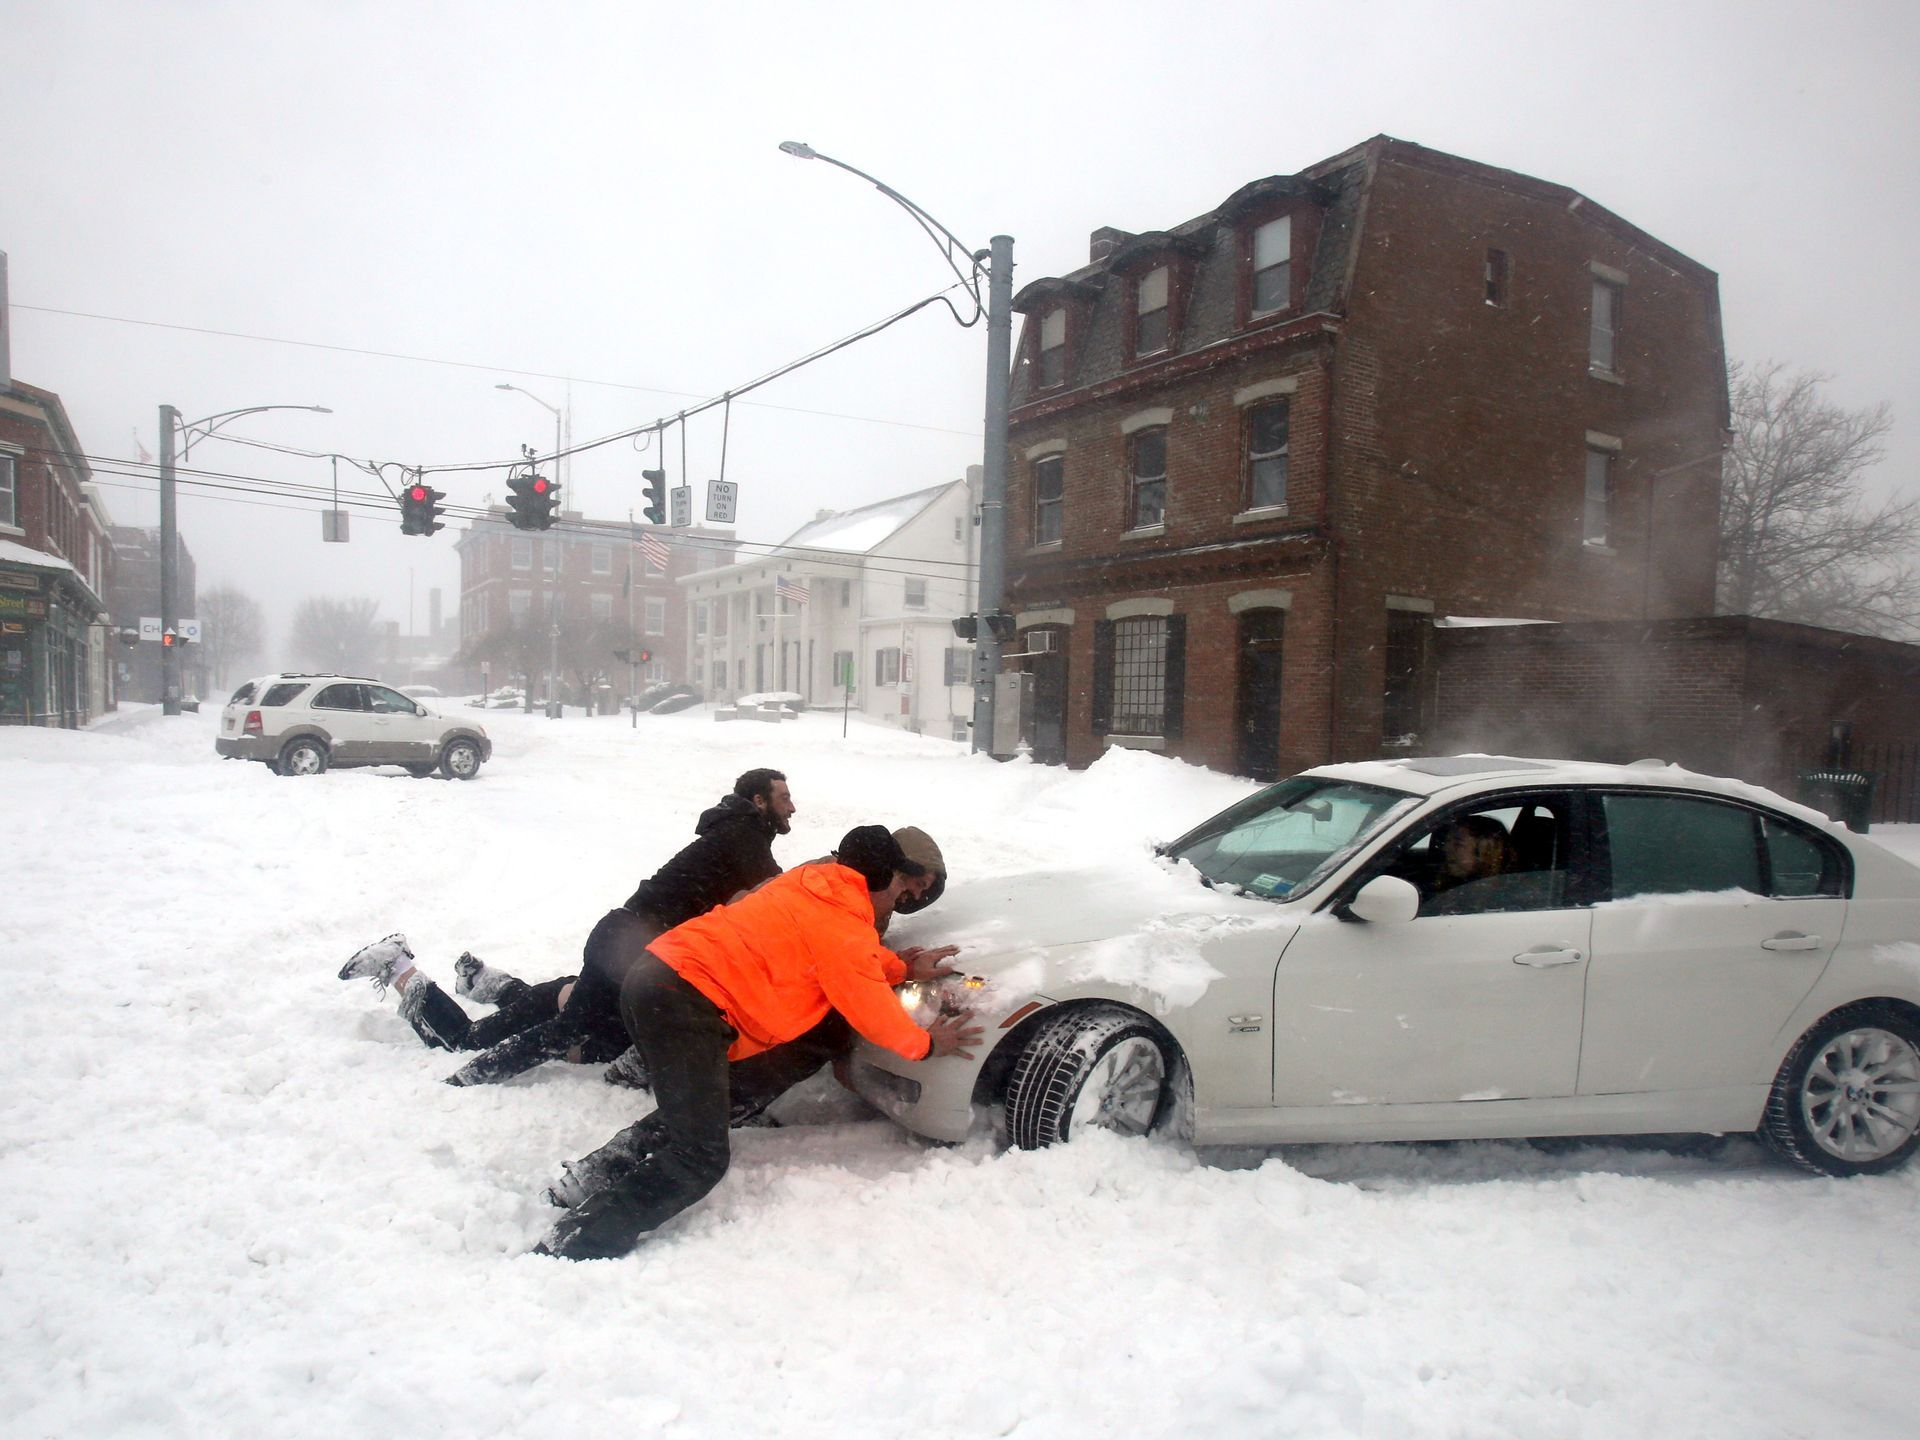
\includegraphics[height=.85\textheight]{snow.jpg}\\
        \footnotesize
        \textit{Copyright Seth Harrison/The Poughkeepsie Journal March 14, 2017}
    \end{center}
\end{frame}

\begin{frame}
    \frametitle{Room Layout}
    \begin{center}
    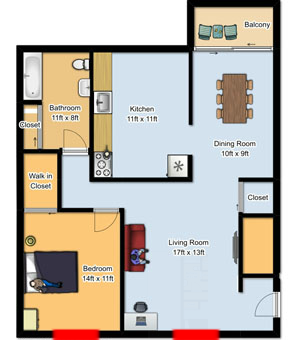
\includegraphics[height=.85\textheight]{floorplan.png}
    \end{center}
\end{frame}

\begin{frame}
    \frametitle{Air Conditioner Units}
    \begin{center}
        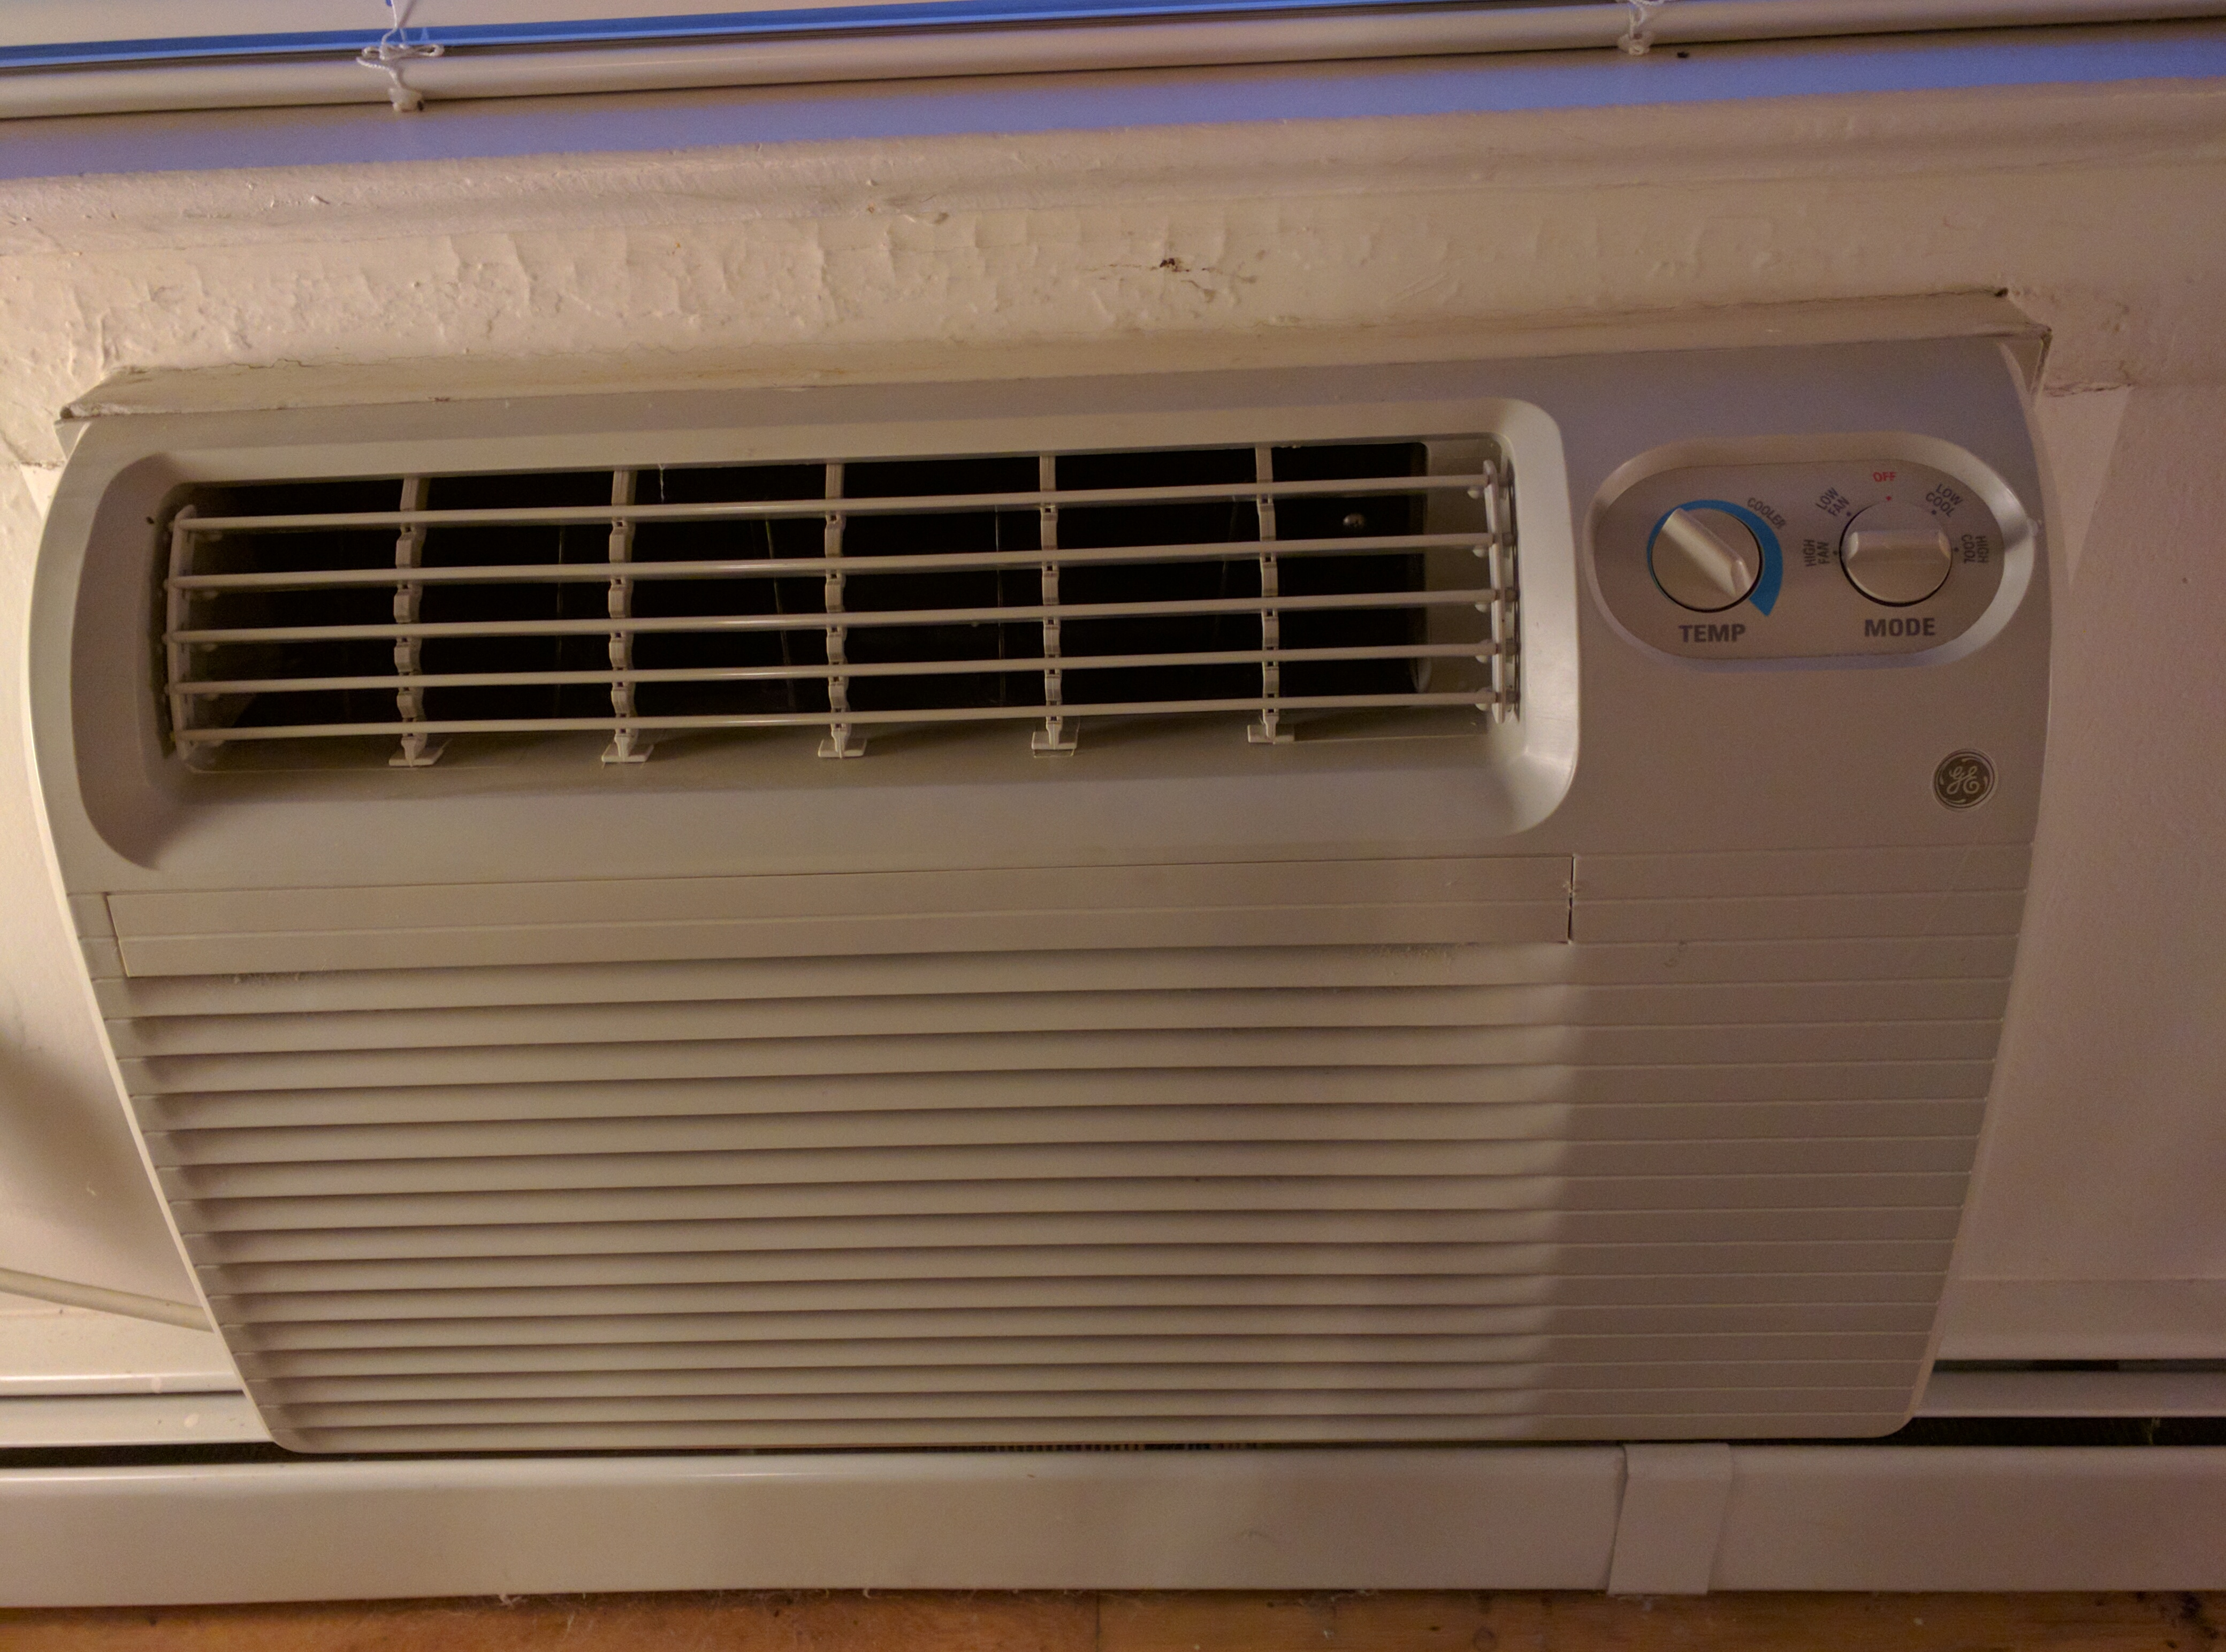
\includegraphics[width=.75\textwidth]{AC_unit.jpeg}
    \end{center}
\end{frame}

\section{Builing a Thermostat}

\begin{frame}
    \frametitle{Thermostat}
    \begin{center}
    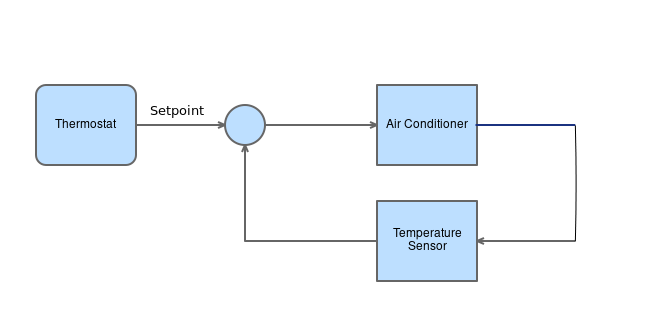
\includegraphics[width=.8\textwidth]{flowchart.png}
    \end{center}
    \begin{itemize}
        \item Closed Loop control device
        \item 1 input temperature sensor
        \item 1 output for controlling heating and/or cooling system
    \end{itemize}
\end{frame}

\subsection{Controlling the AC}
\begin{frame}
    \frametitle{Constraints for controlling the AC}
    \begin{center}
        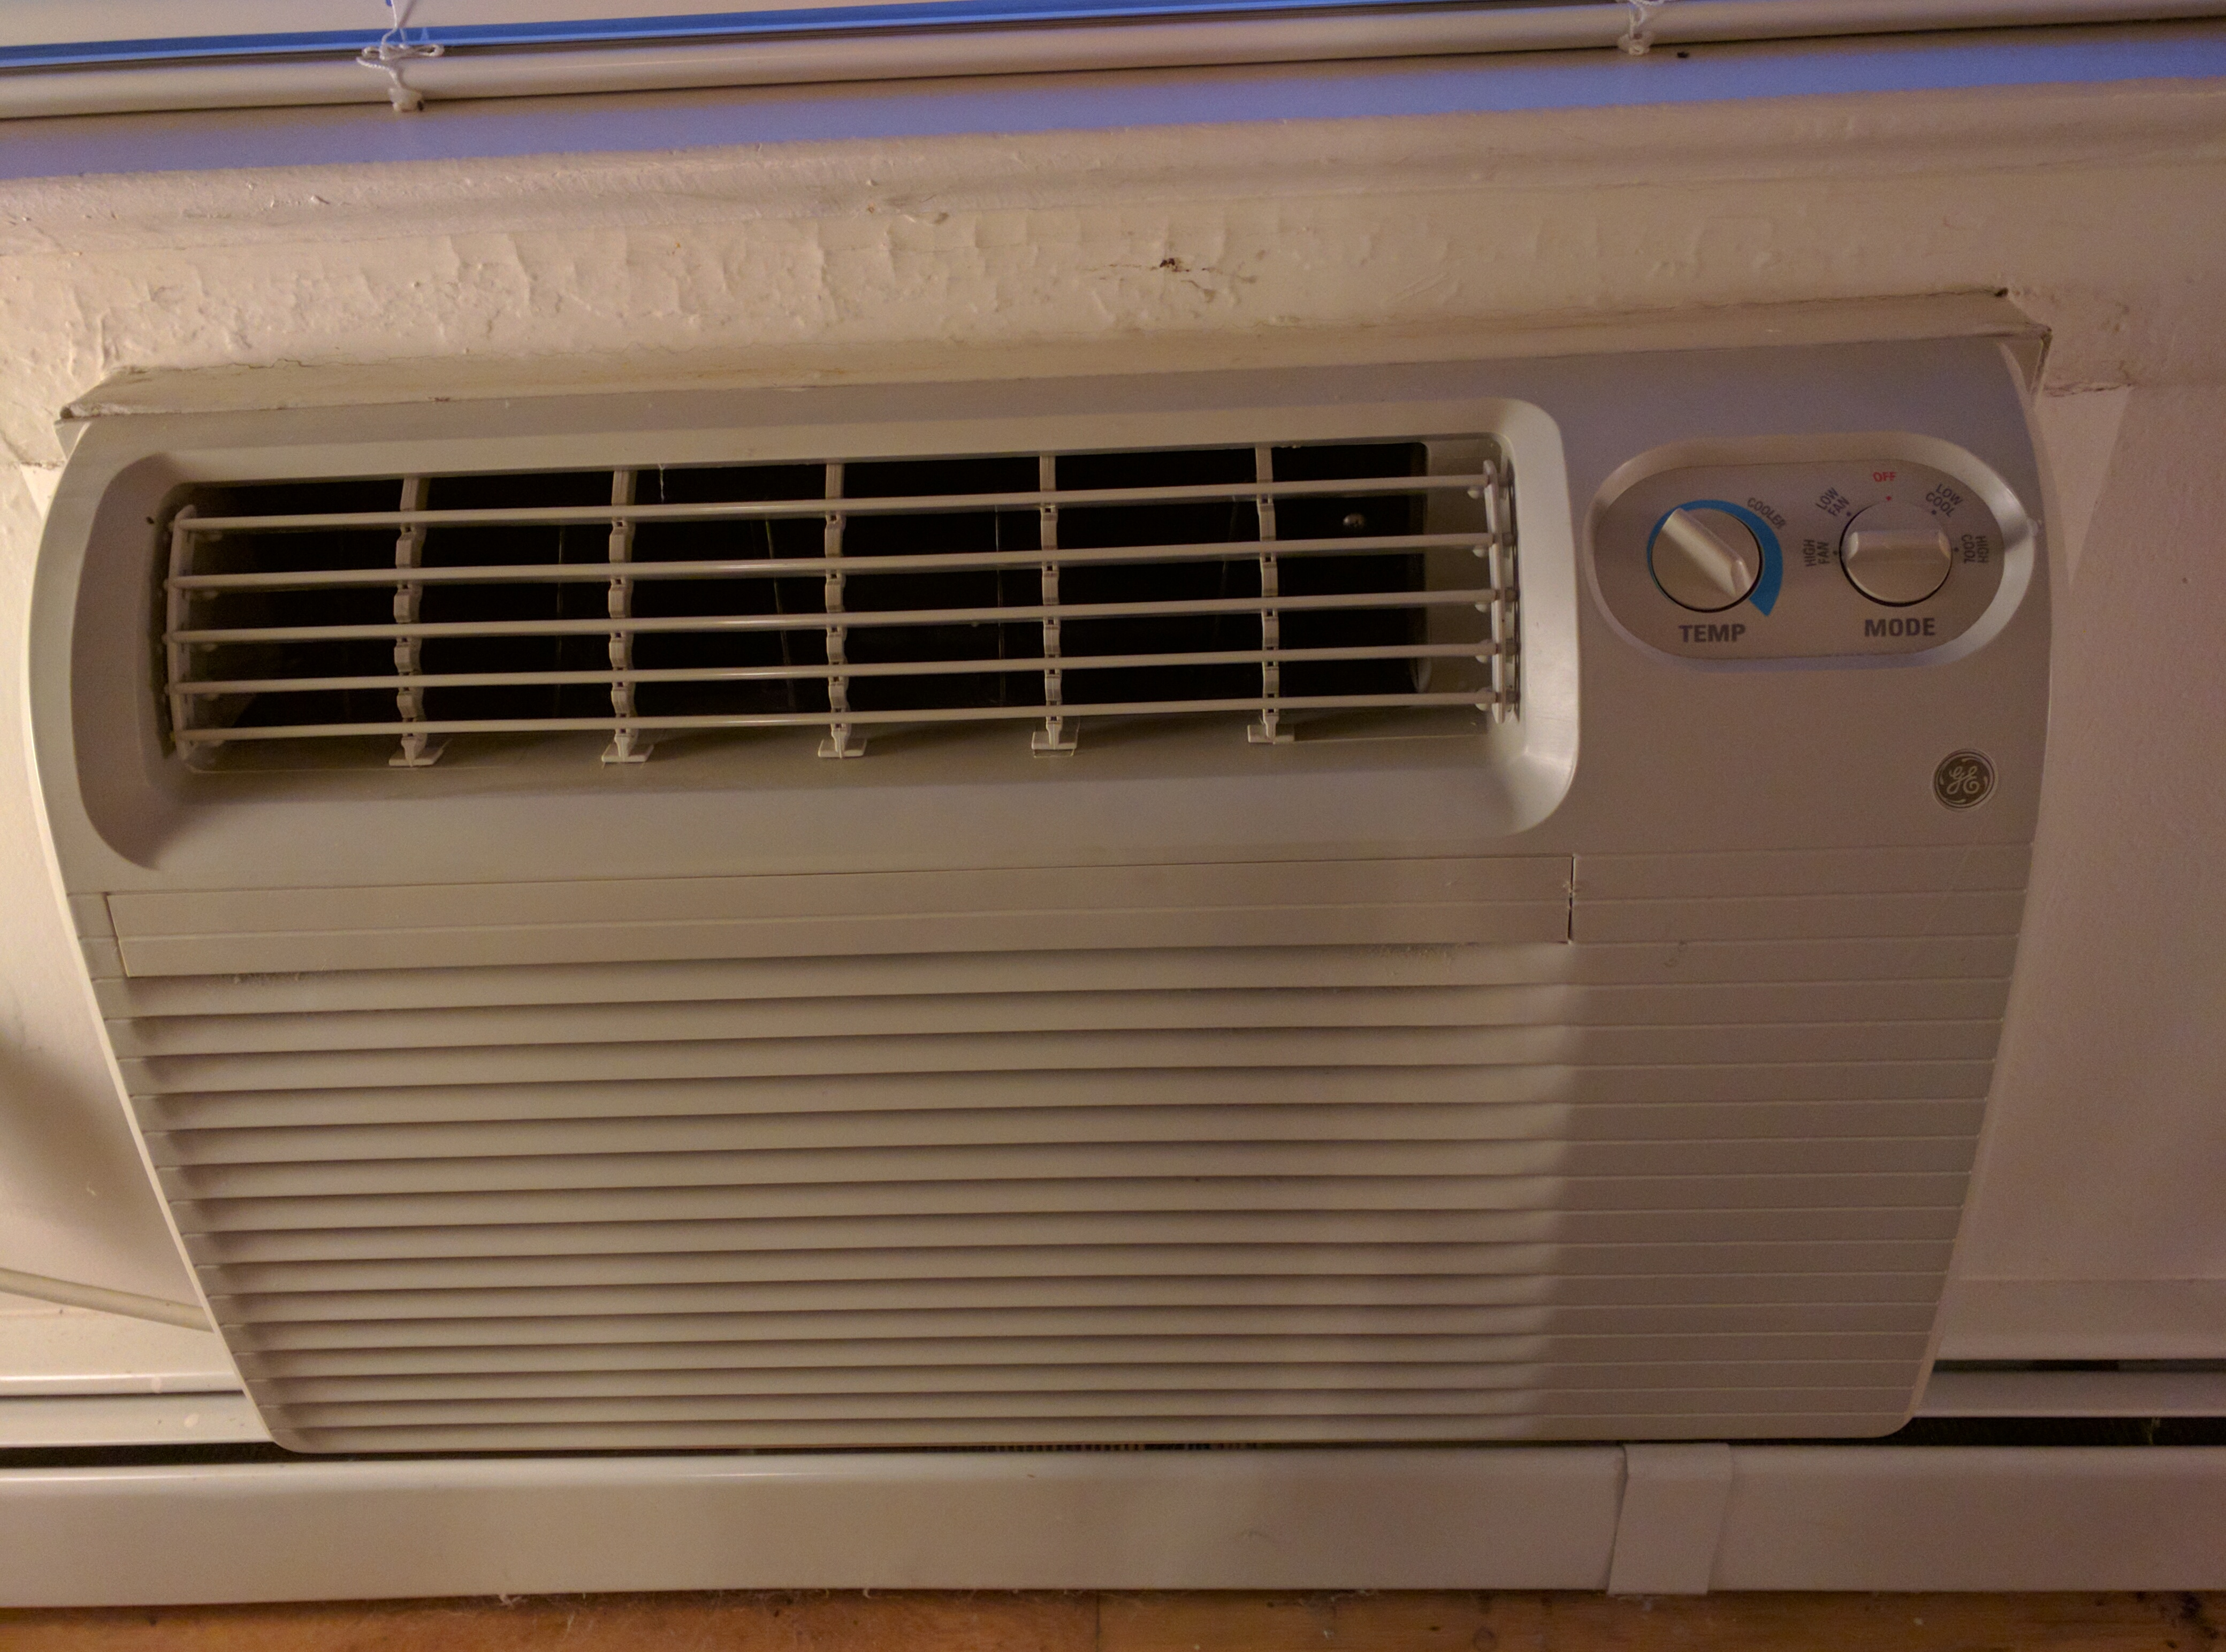
\includegraphics[width=.53\textwidth]{AC_unit.jpeg}
    \end{center}
    \begin{itemize}
        \item Can't take apart the Air Conditioner (I don't own it)
        \item No identifying information for the AC
        \item Wireless control is ideal
    \end{itemize}
\end{frame}

\begin{frame}
    \frametitle{Solution for controlling the AC}
    \begin{columns}
        \begin{column}{.48\textwidth}
            \begin{itemize}
                \item Control via power (use a relay to turn on and off)
                \item Measured current draw with clamp meter
                \item Purchased a Z-Wave power switch
            \end{itemize}
        \end{column}
        \begin{column}{.48\textwidth}
            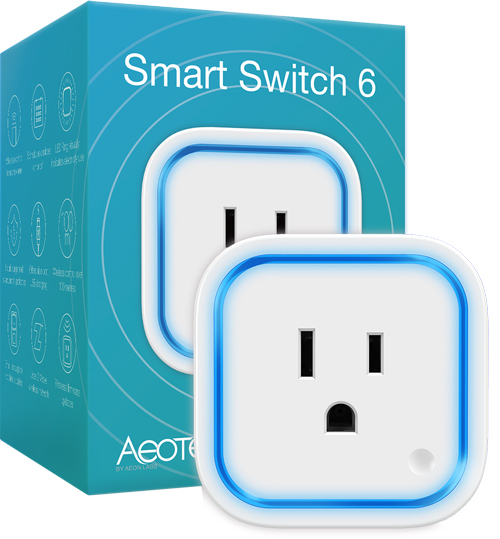
\includegraphics[width=.8\textwidth]{aeotec-ss6.jpg}
        \end{column}
    \end{columns}
\end{frame}

\subsection{Z-Wave}
\begin{frame}
    \frametitle{What is Z-Wave}
    \begin{columns}
        \begin{column}{.48\textwidth}
            \begin{itemize}
                \item Low power mesh network for sensors and devices
                \item Licensed by Sigma Designs
                \item Interoperability tested for all devices by Z-Wave Alliance
                \item Software API and protocol docs in the public domain
                \item Over 1700 certified devices
                \item OpenZwave is an Open Source library to interface with a Z-Wave network
            \end{itemize}
        \end{column}
        \begin{column}{.48\textwidth}
            
\includegraphics[width=\textwidth]{zwave.png}
        \end{column}
    \end{columns}
\end{frame}

\subsection{Temperature Sensing}
\begin{frame}
    \frametitle{Sensing the Temperature}
    \begin{columns}
        \begin{column}{.48\textwidth}
            \begin{itemize}
                \item Wireless sensor
                \item Leverage the new Z-Wave network
                \item Purchased a Z-Wave multi sensor which included temperature
            \end{itemize}
        \end{column}
        \begin{column}{.48\textwidth}
            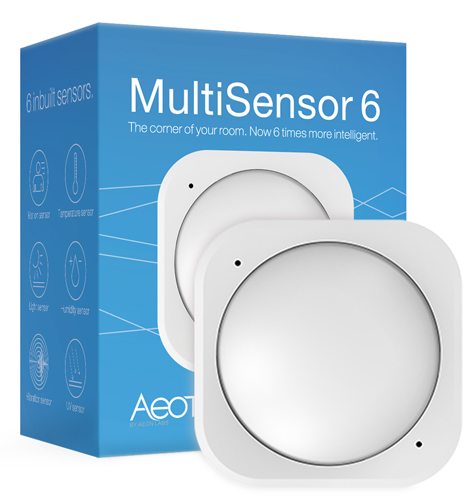
\includegraphics[width=\textwidth]{aeotec-multi.jpg}
        \end{column}
    \end{columns}
\end{frame}

\begin{frame}
    \frametitle{Using Z-Wave}
    \begin{columns}[T]
        \begin{column}{.48\textwidth}
            \begin{itemize}
                \item Setup a Z-Wave network with Aeotec Z-Stick
                \item Register each device on the network
                \item Leverage OpenZWave to provide an API to interact with
                    devices
            \end{itemize}
        \end{column}
        \begin{column}{.48\textwidth}
            \centering
            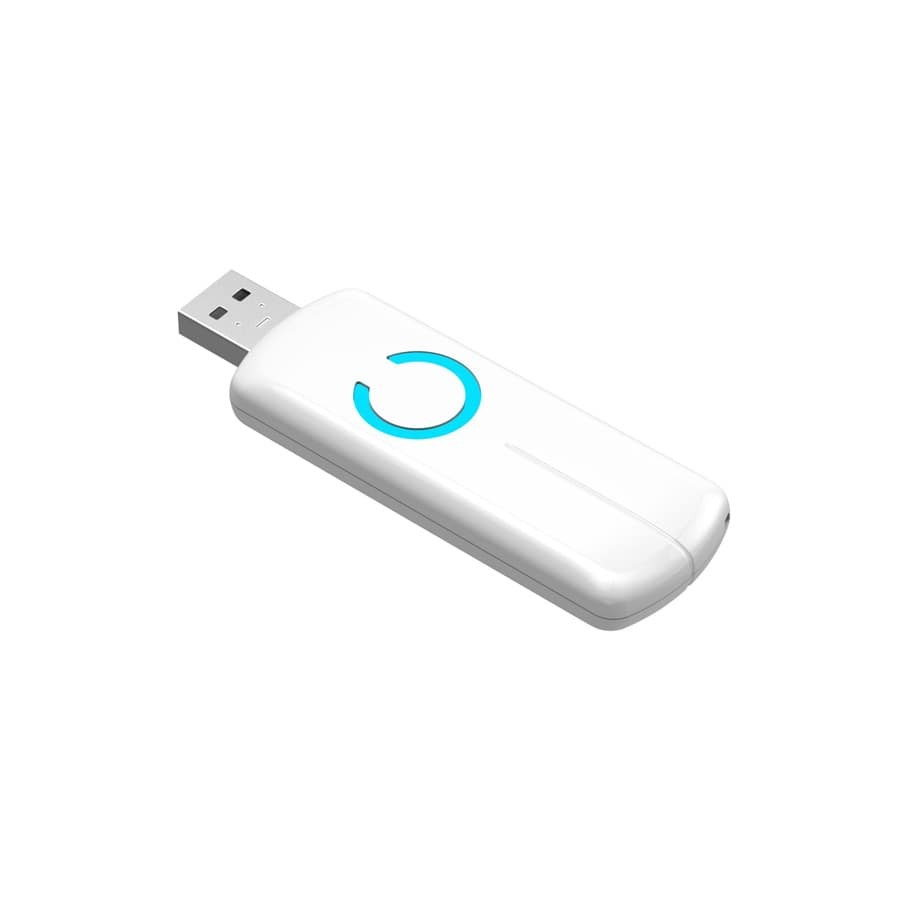
\includegraphics[width=.8\textwidth]{aeotec-zstick.jpg}
        \end{column}
    \end{columns}
\end{frame}

\subsection{Software}
\begin{frame}
    \frametitle{Home Assistant}
    \begin{columns}
        \begin{column}{.48\textwidth}
            \begin{itemize}
                \item Open Source Home Automation Platform
                \item Written in Python 3
                \item Has over 900 different components
                \item Runs locally (with all data stored locally)
                \item Design point that it will always run on Raspberry Pi 3
            \end{itemize}
        \end{column}
        \begin{column}{.48\textwidth}
            
\includegraphics[width=\textwidth]{homeassistant.png}
        \end{column}
    \end{columns}
\end{frame}

\begin{frame}
    \frametitle{Home Assistant in Practice}
    \centering
    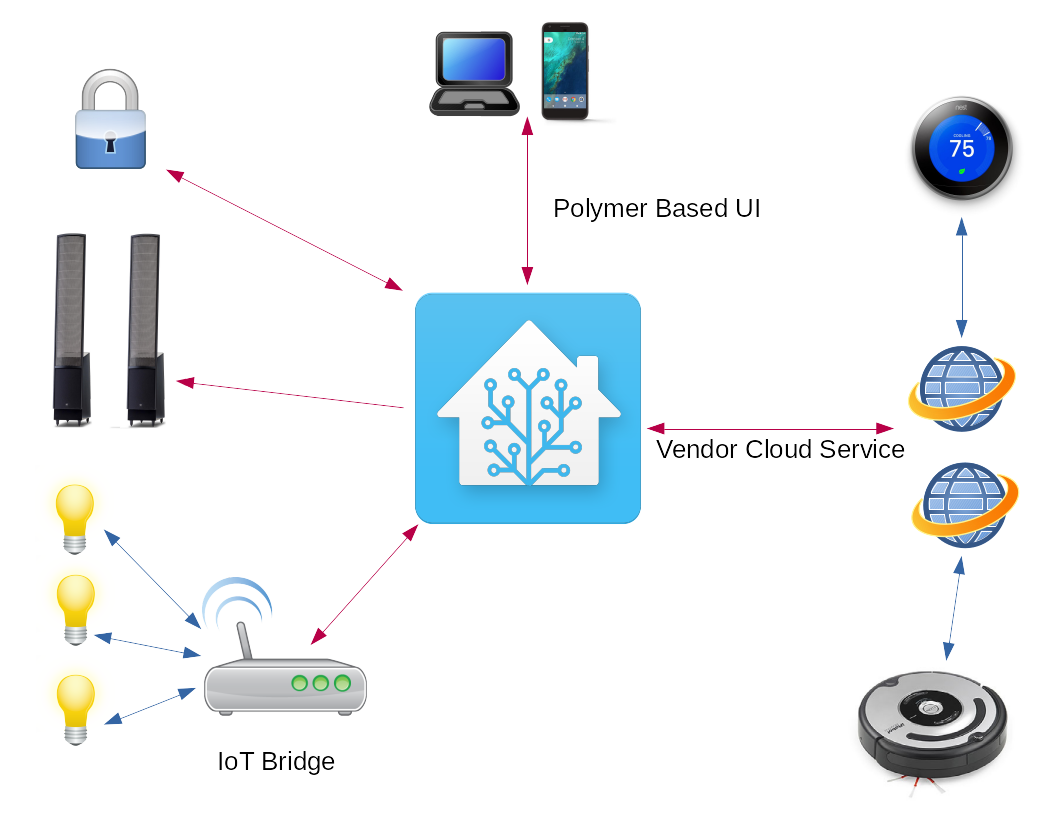
\includegraphics[height=.95\textheight]{HA_in_practice.png}

\end{frame}

\begin{frame}
    \frametitle{Internal Architecture}
    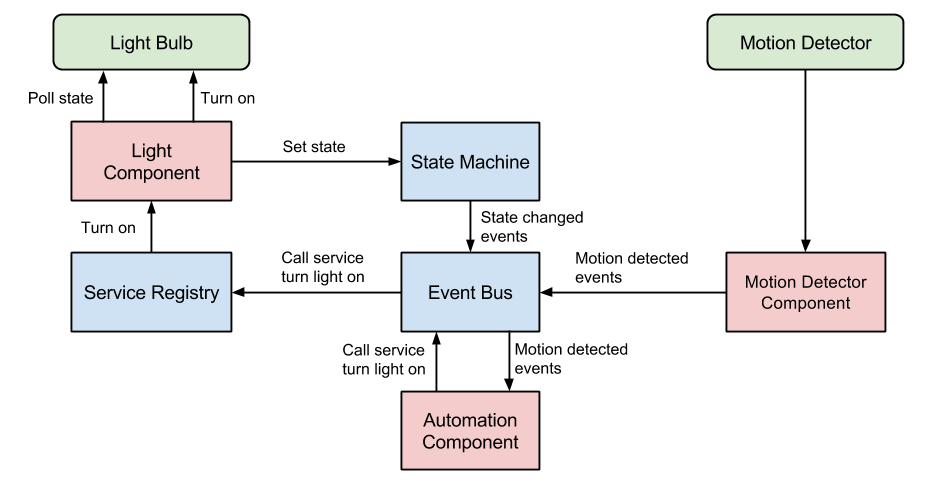
\includegraphics[width=\textwidth]{state_machine.png}
\end{frame}

\begin{frame}[fragile=singleslide]
    \frametitle{First Attempt at a thermostat}
    \begin{minted}[
        gobble=4,
        frame=single,
        fontsize=\small,
        linenos
    ]{yaml}
      alias: Turn off Living Room AC when below 25 C
      trigger:
        platform: numeric_state
        entity_id: sensor.aeotec_zw100_multisensor_6_temperature_4
        below: 25
      condition:
        - condition: state
          entity_id: switch.aeotec_zw096_smart_switch_6_switch_2
          state: 'on'
          for:
            minutes: 20
      action:
        service: switch.turn_off
        entity_id: switch.aeotec_zw096_smart_switch_6_switch_2
    \end{minted}
\end{frame}

\begin{frame}
    \frametitle{Issues with this approach}
    \begin{itemize}
        \item Requires writing a separate rule for ever possible condition
        \item Rules only triggered on state updates
        \item Switching became unreliable
        \item Adjusting the set point required a configuration update
    \end{itemize}
\end{frame}

\begin{frame}
    \frametitle{Setting up a thermostat device in Home Assistant}
    \begin{columns}[T]
        \begin{column}{.48\textwidth}
            \begin{center}
                \href{https://home-assistant.io/components/\#climate}{https://home-assistant.io/components/\#climate}
                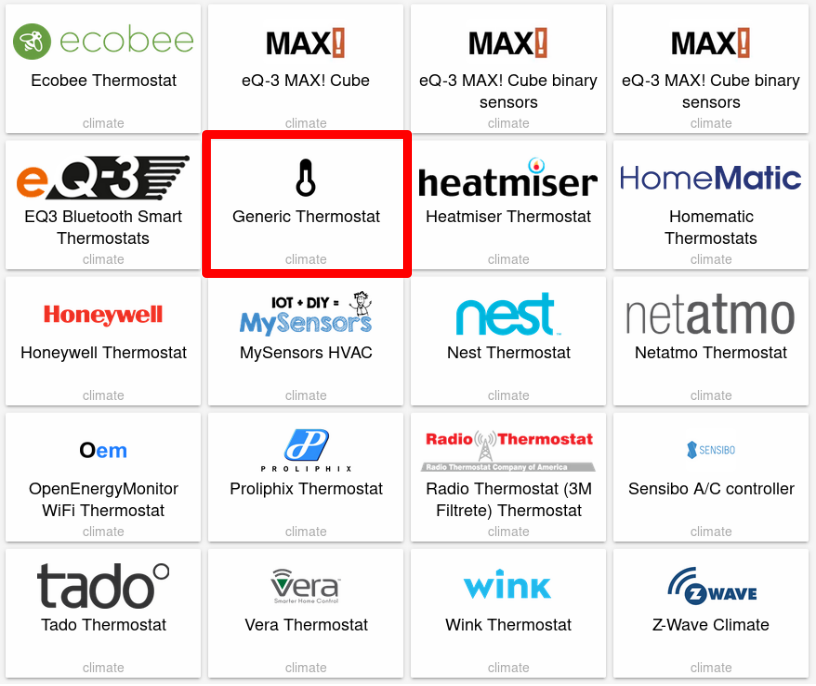
\includegraphics[width=\textwidth]{thermostat_components_2.png}
            \end{center}
        \end{column}
        \begin{column}{.48\textwidth}
            \begin{itemize}
                \item Many thermostat modules depending on hardware
                \item The generic thermostat component exists to run it in
                    software
                \item In the component configuration define a generic thermostat
                    devices with a temperature sensor and switch
            \end{itemize}
        \end{column}
    \end{columns}
\end{frame}

\begin{frame}[fragile=singleslide]
    \frametitle{Configuring a software thermostat in Home Assistant}
    \begin{minted}[
        gobble=4,
        frame=single,
        fontsize=\small,
        linenos
    ]{yaml}
      climate:
        - name: Living Room
          platform: generic_thermostat
          heater: switch.aeotec_smart_switch_6_switch_5_0
          target_sensor: sensor.aeotec_zw100_multisensor_6_temperature_4_1
          min_temp: 20
          max_temp: 35
          target_temp: 25
          ac_mode: True
    \end{minted}
\end{frame}


\begin{frame}
    \frametitle{Home Assistant Web Dashboard}
    \begin{columns}
        \begin{column}{.48\textwidth}
            \begin{center}
                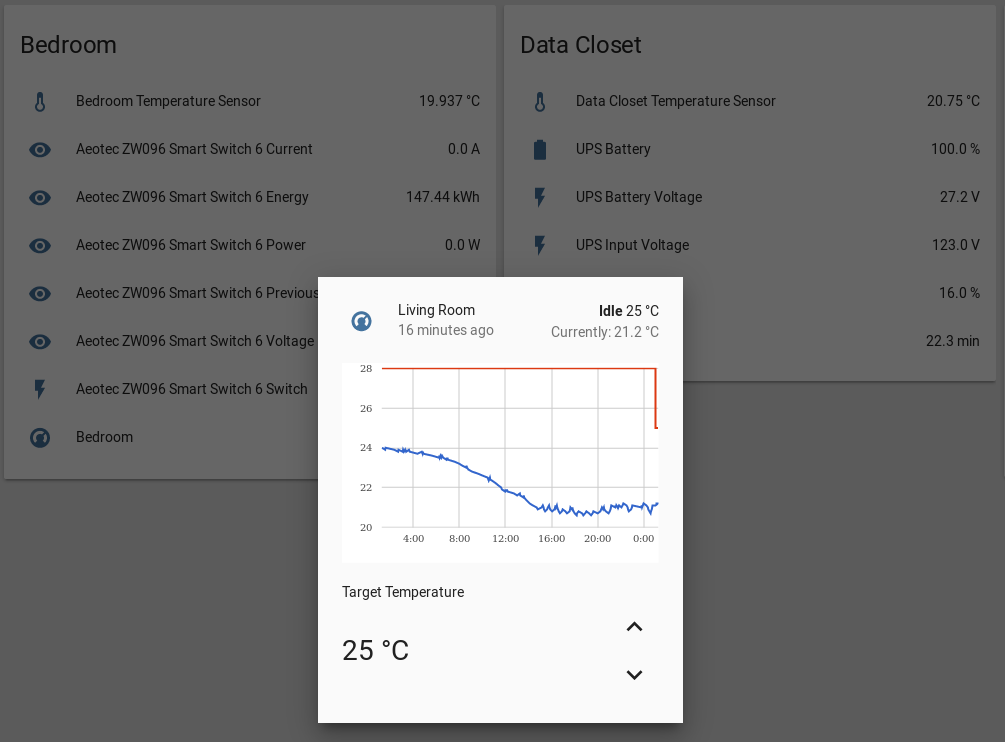
\includegraphics[width=1.2\textwidth]{Control_panel_trimmed.png}
            \end{center}
        \end{column}
        \begin{column}{.48\textwidth}
            \begin{center}
                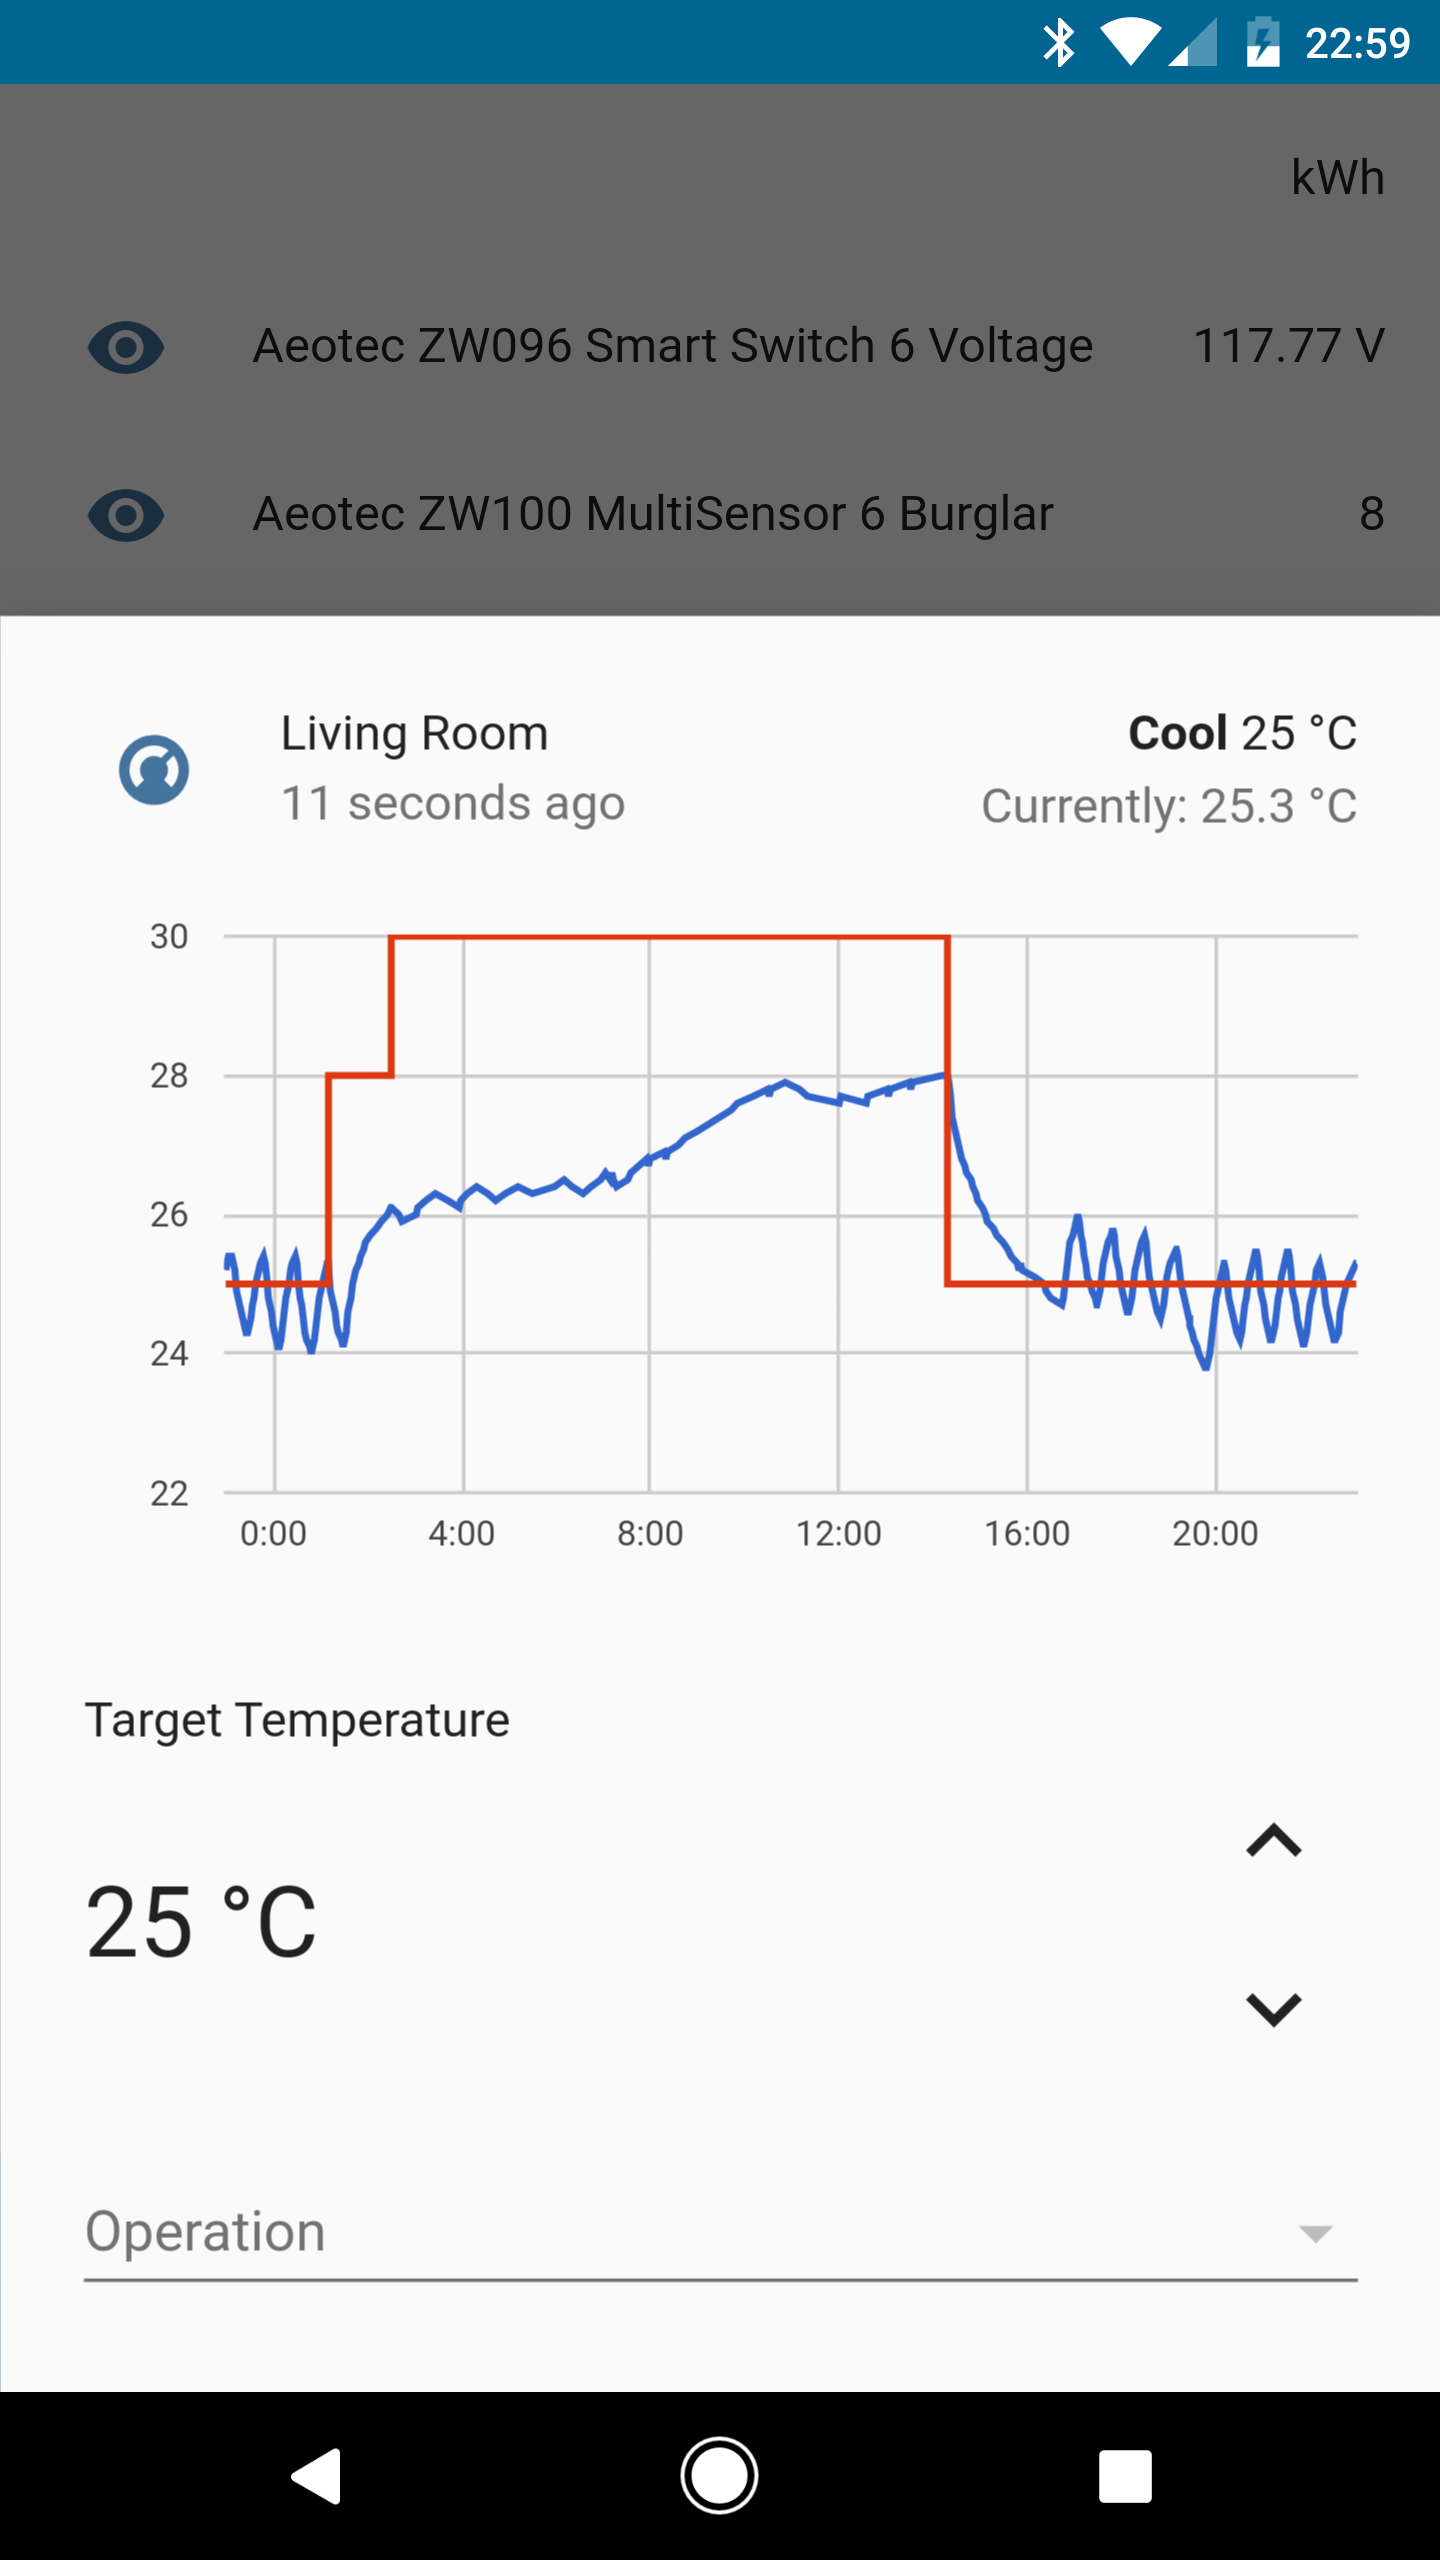
\includegraphics[width=.62\textwidth]{mobile_interface.png}
            \end{center}
        \end{column}
    \end{columns}
\end{frame}

\section{Initial Problems}
\subsection{Making it multizone}
\begin{frame}
    \frametitle{Problems with this\dots}
    \begin{center}
    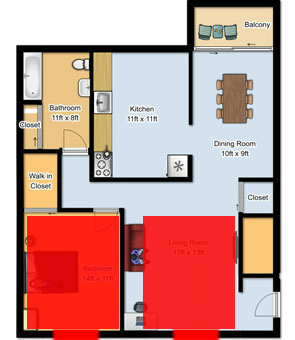
\includegraphics[height=.85\textheight]{floorplan-zones.png}
    \end{center}
\end{frame}

\subsubsection{Bedroom Temperature Sensing}
\begin{frame}
    \frametitle{Bedroom Temperature Sensing}
    \begin{columns}[T]
        \begin{column}{.48\textwidth}
            \begin{itemize}
                \item Track both bedroom and ``data`` closet temperatures
                \item Leverage spare Raspberry Pi sitting in ``data'' closet
                \item 2x DS18B20 Dallas 1 wire temperature sensors used
            \end{itemize}
        \end{column}
        \begin{column}{.48\textwidth}
            \centering
            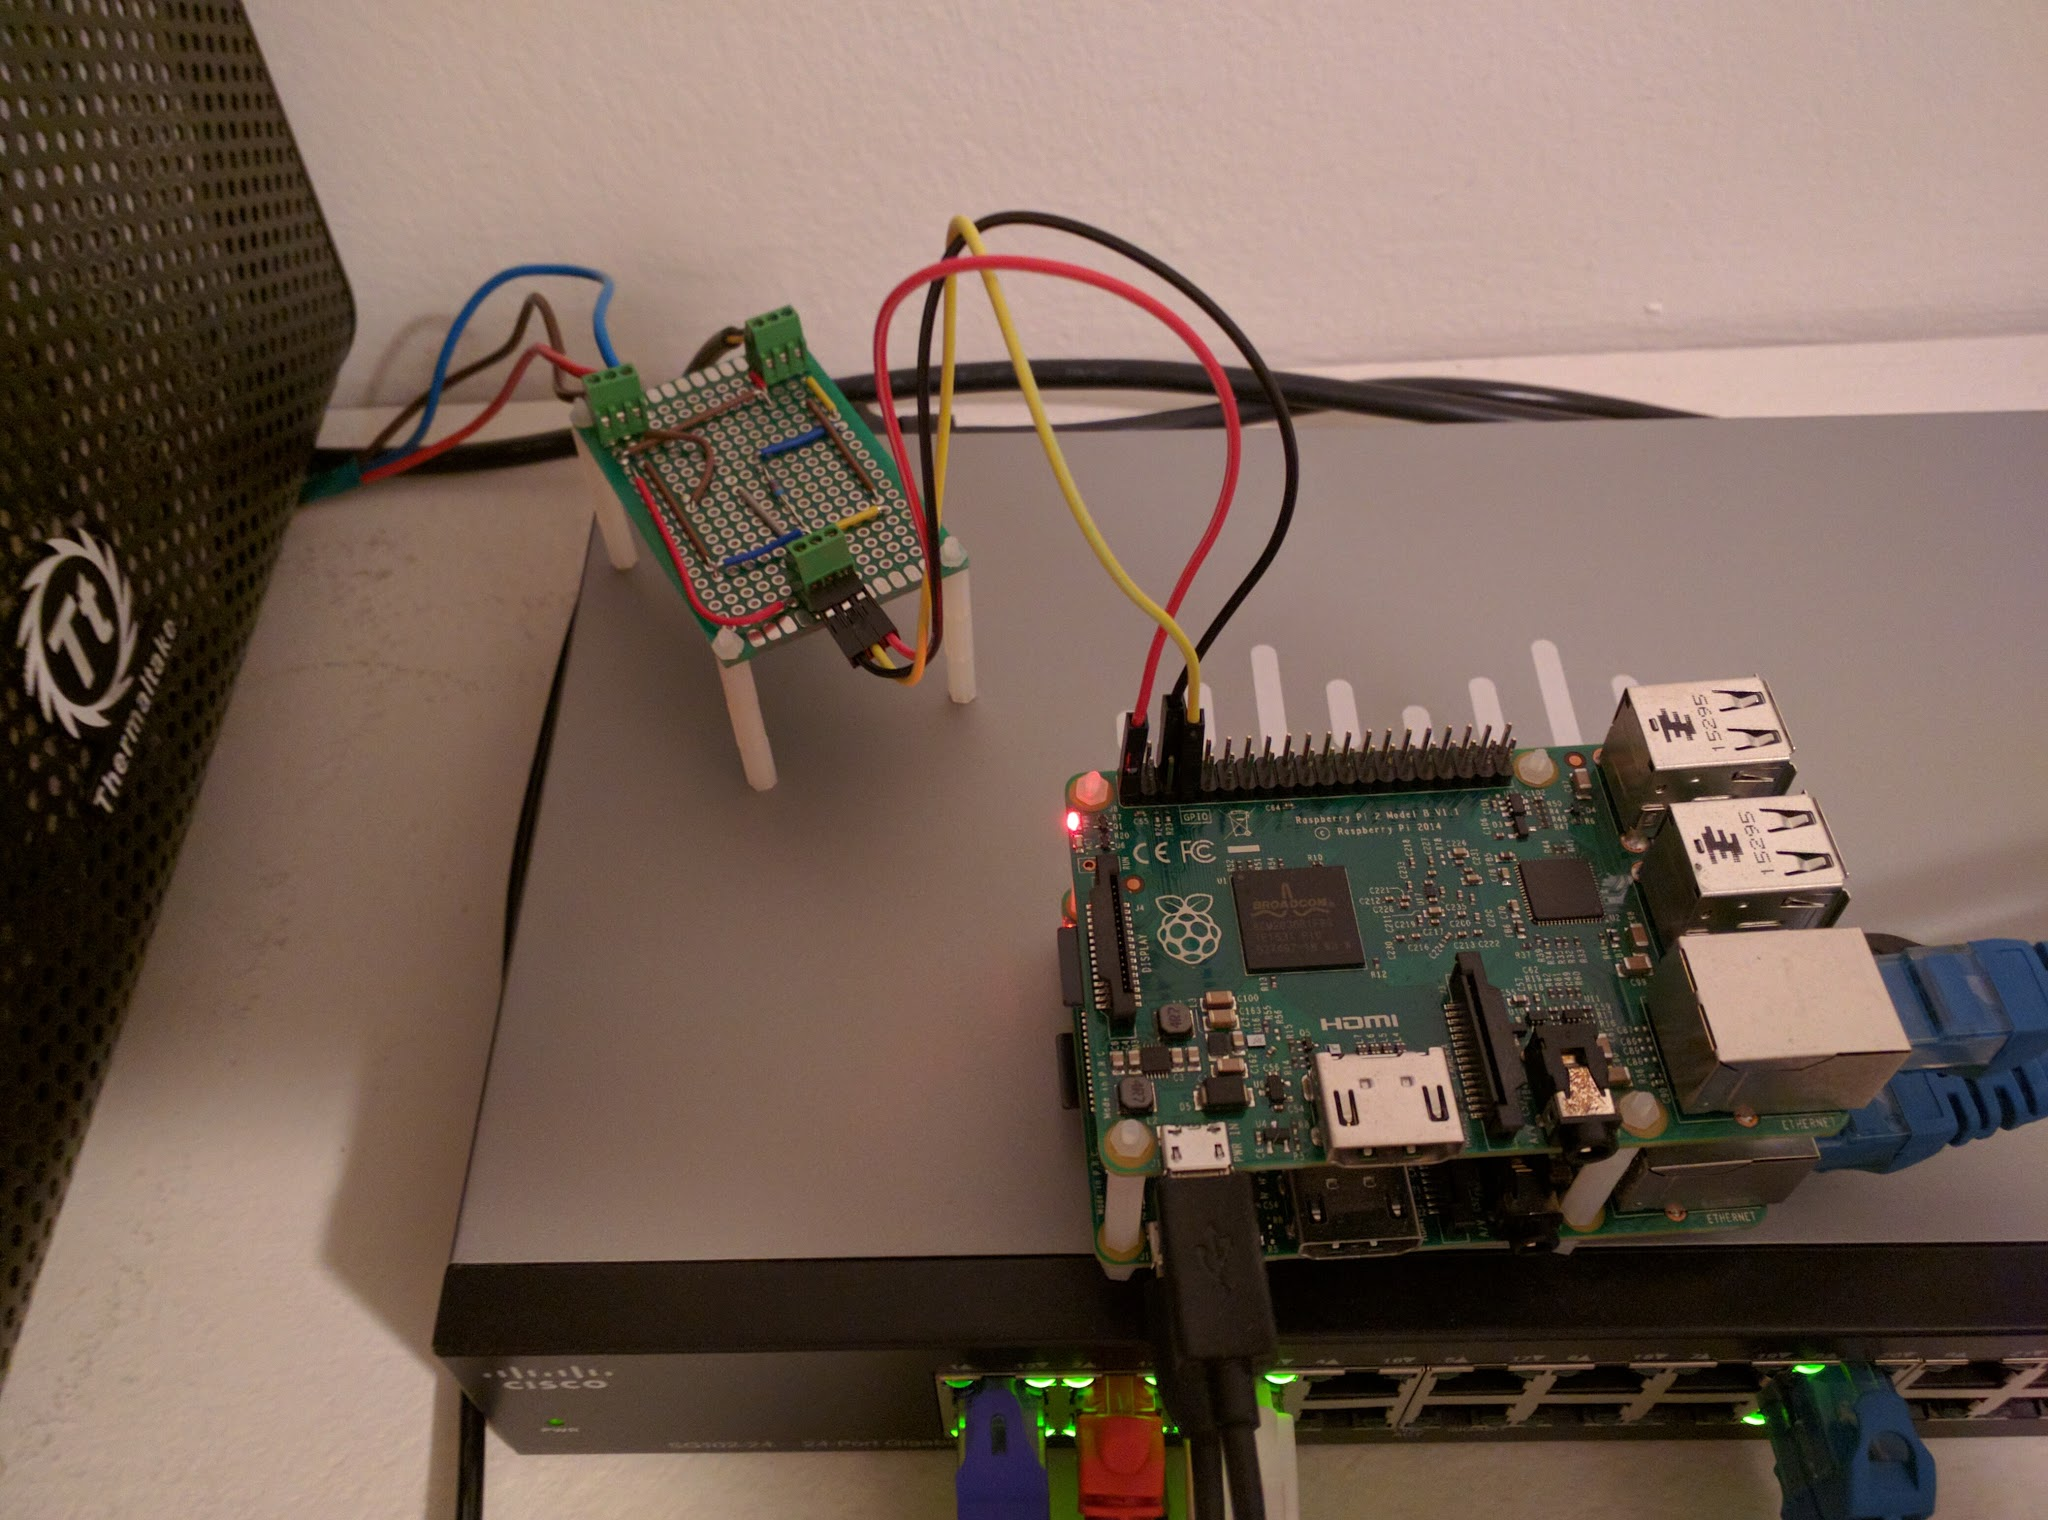
\includegraphics[width=\textwidth]{raspi.jpg}
        \end{column}
    \end{columns}
\end{frame}

\begin{frame}
    \frametitle{Data Closet}
    \centering
    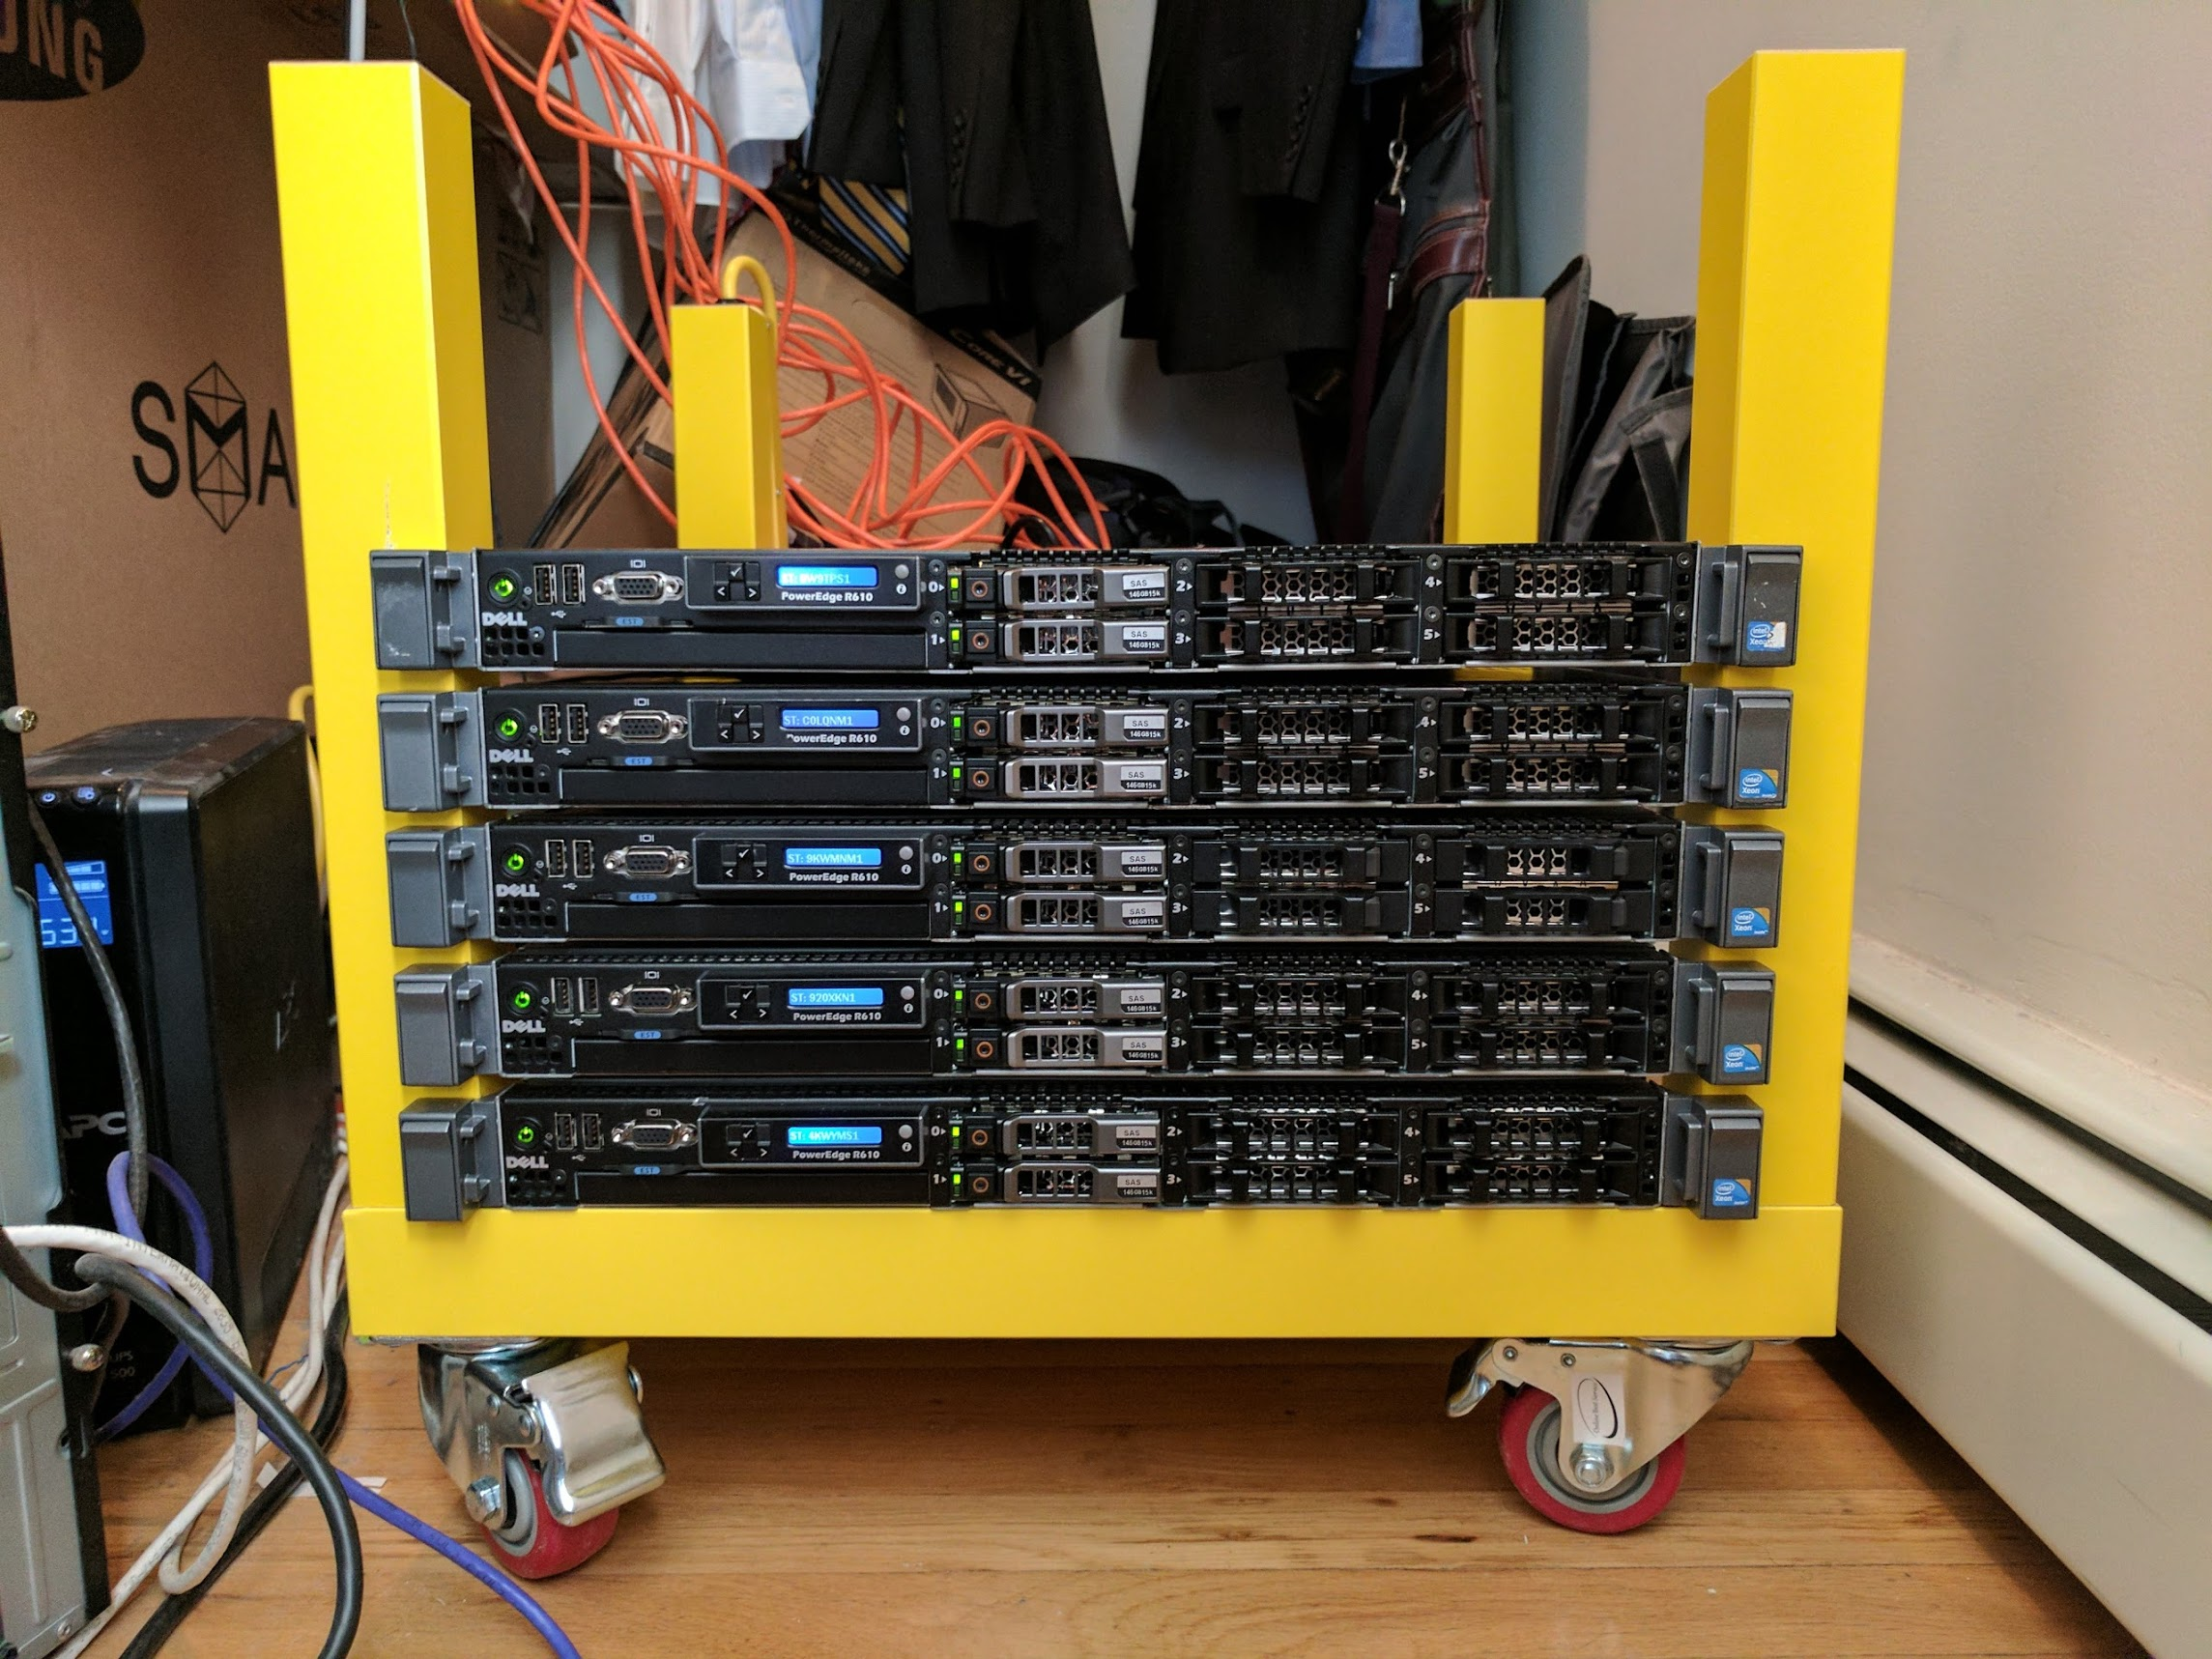
\includegraphics[width=.75\textwidth]{data_closet.jpg}
\end{frame}

\begin{frame}
    \frametitle{DallasMQTT}
    \begin{itemize}
        \item Framework for polling sensors and pushing results on MQTT
        \item Handles an arbitrary number of sensors
        \item Currently only supports Dallas 1 wire temperature sensors from w1\_therm linux driver
        \item Written in python
    \end{itemize}
\end{frame}

\subsection{Cycle Times}
\begin{frame}
    \frametitle{Short Cycle Time}
    \begin{center}
        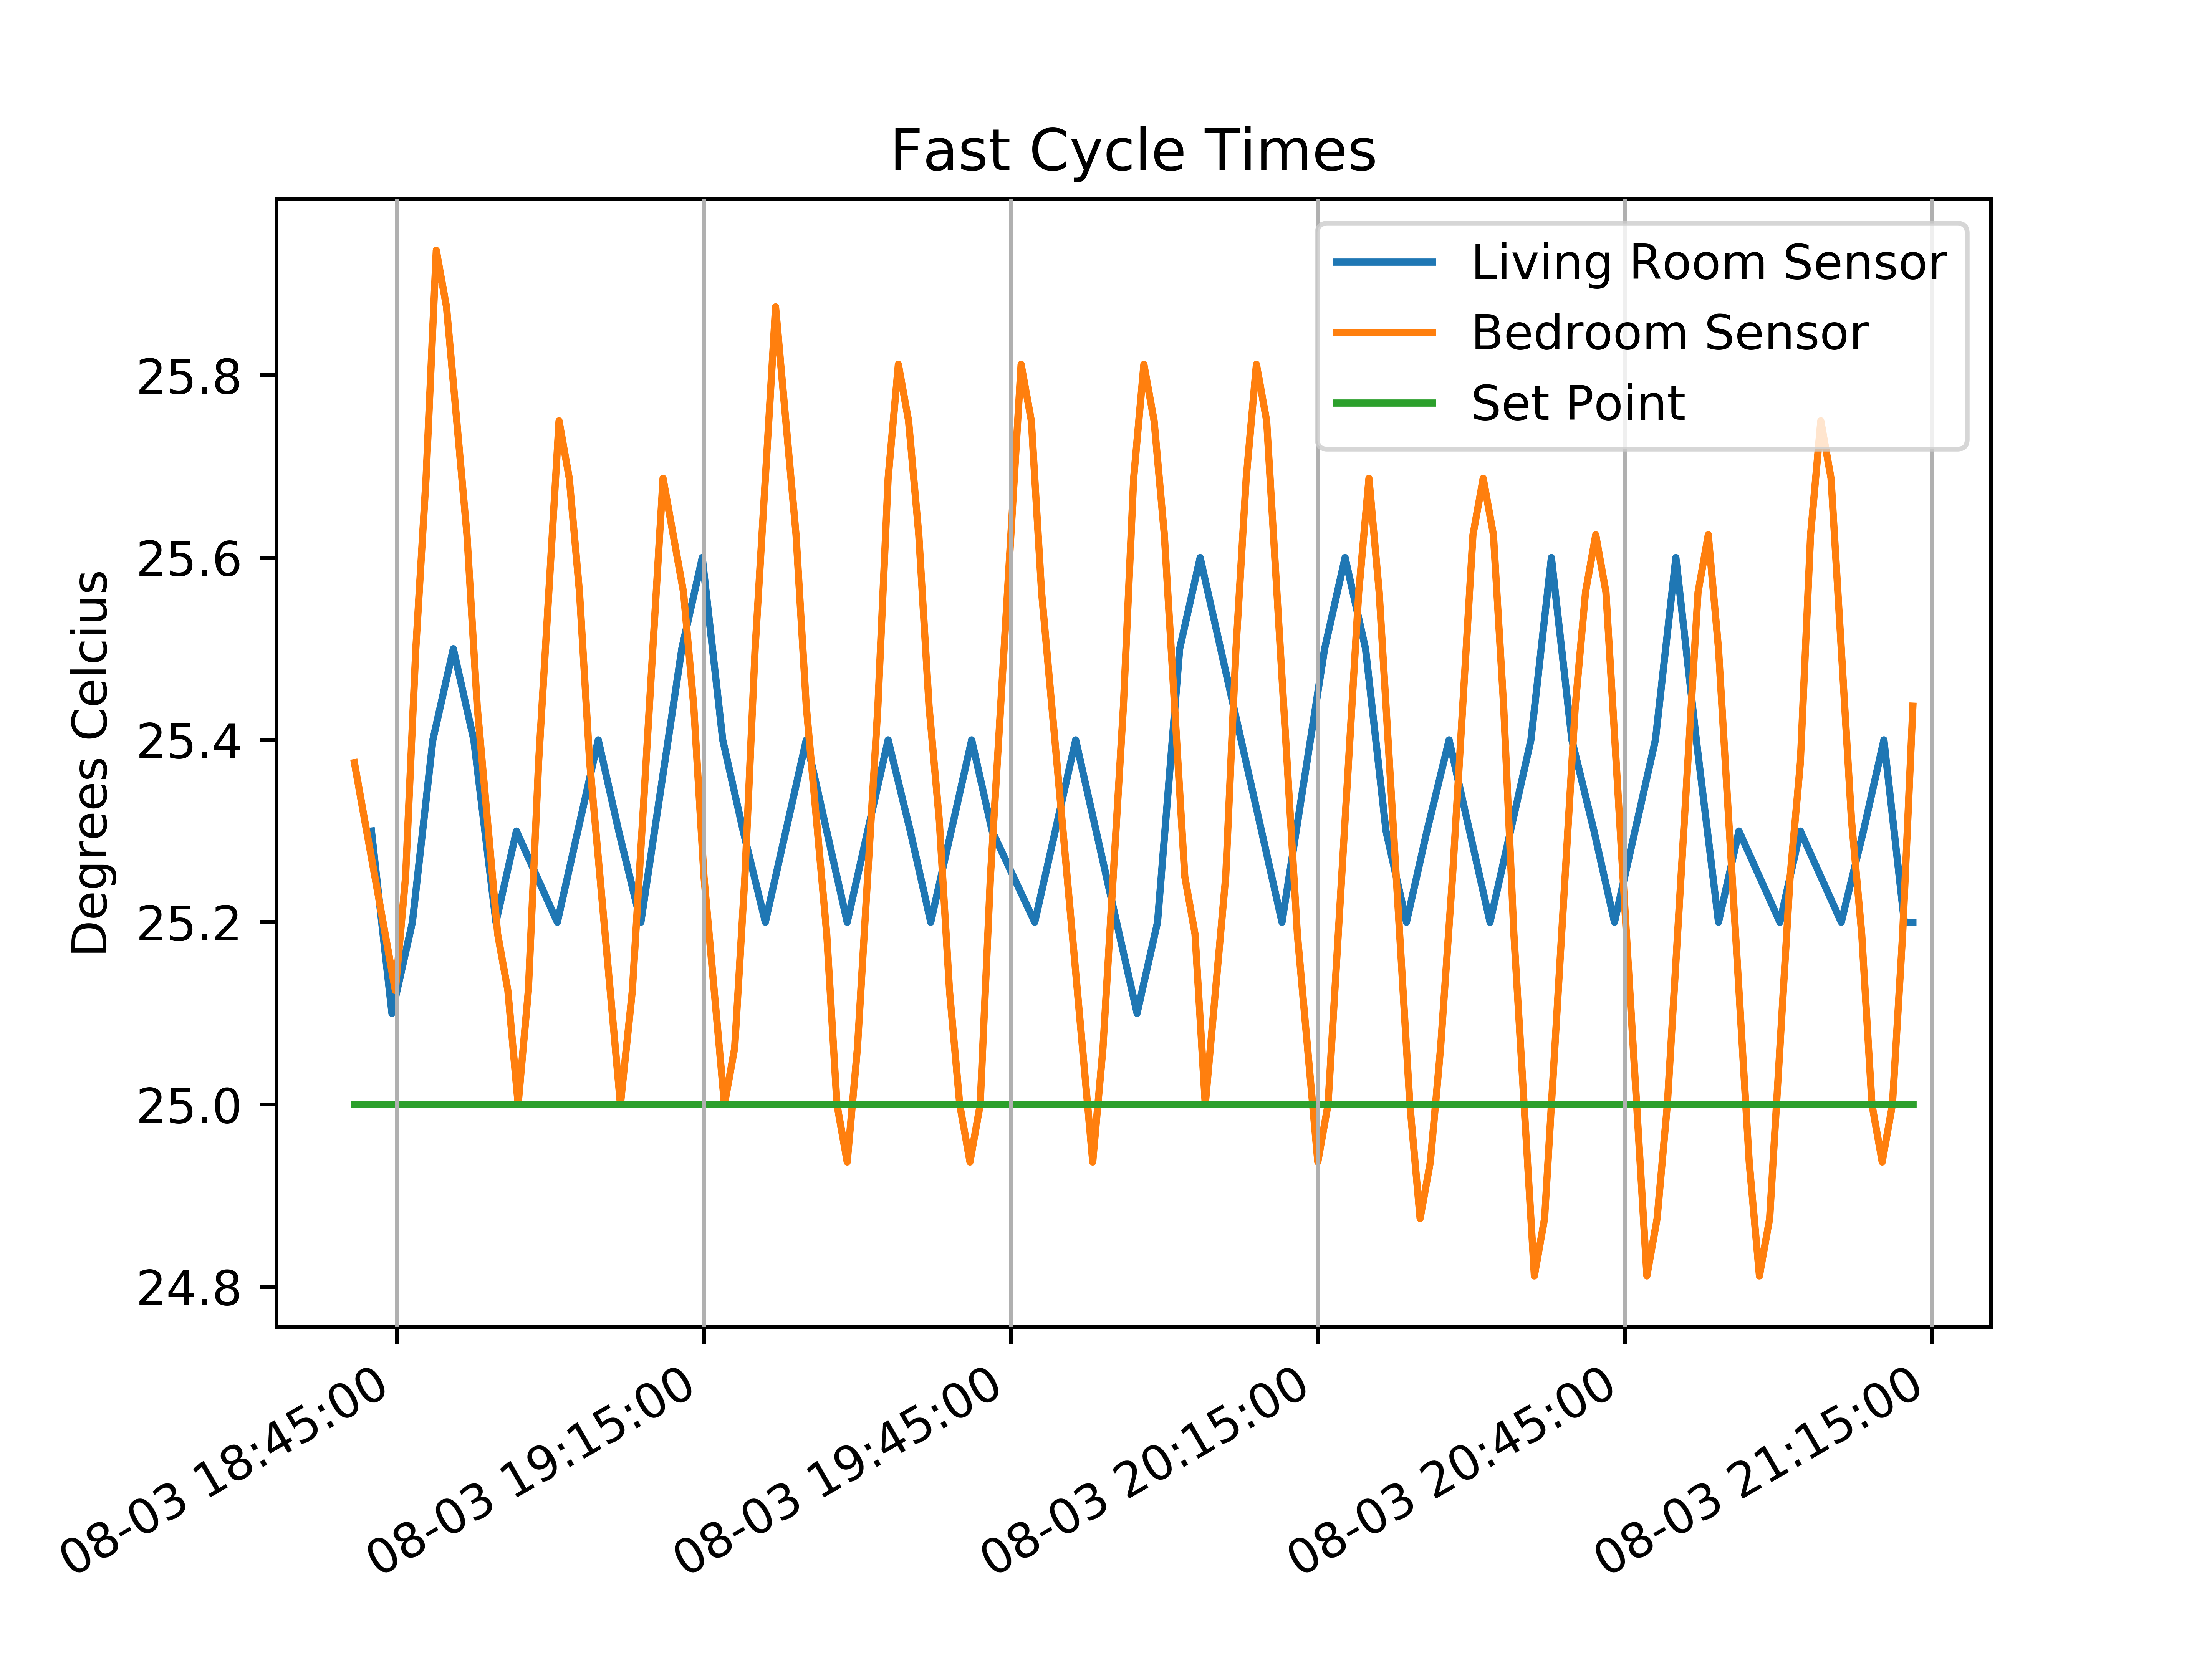
\includegraphics[height=.75\textheight]{short_cycle.png}
    \end{center}
    \begin{itemize}
        \item Bedroom on for 8 min. and off for 4 min.
        \item Living Room on for 4 min. off for 2 min.
    \end{itemize}
\end{frame}

\begin{frame}
    \frametitle{Corrected Cycle Time}
    \begin{center}
        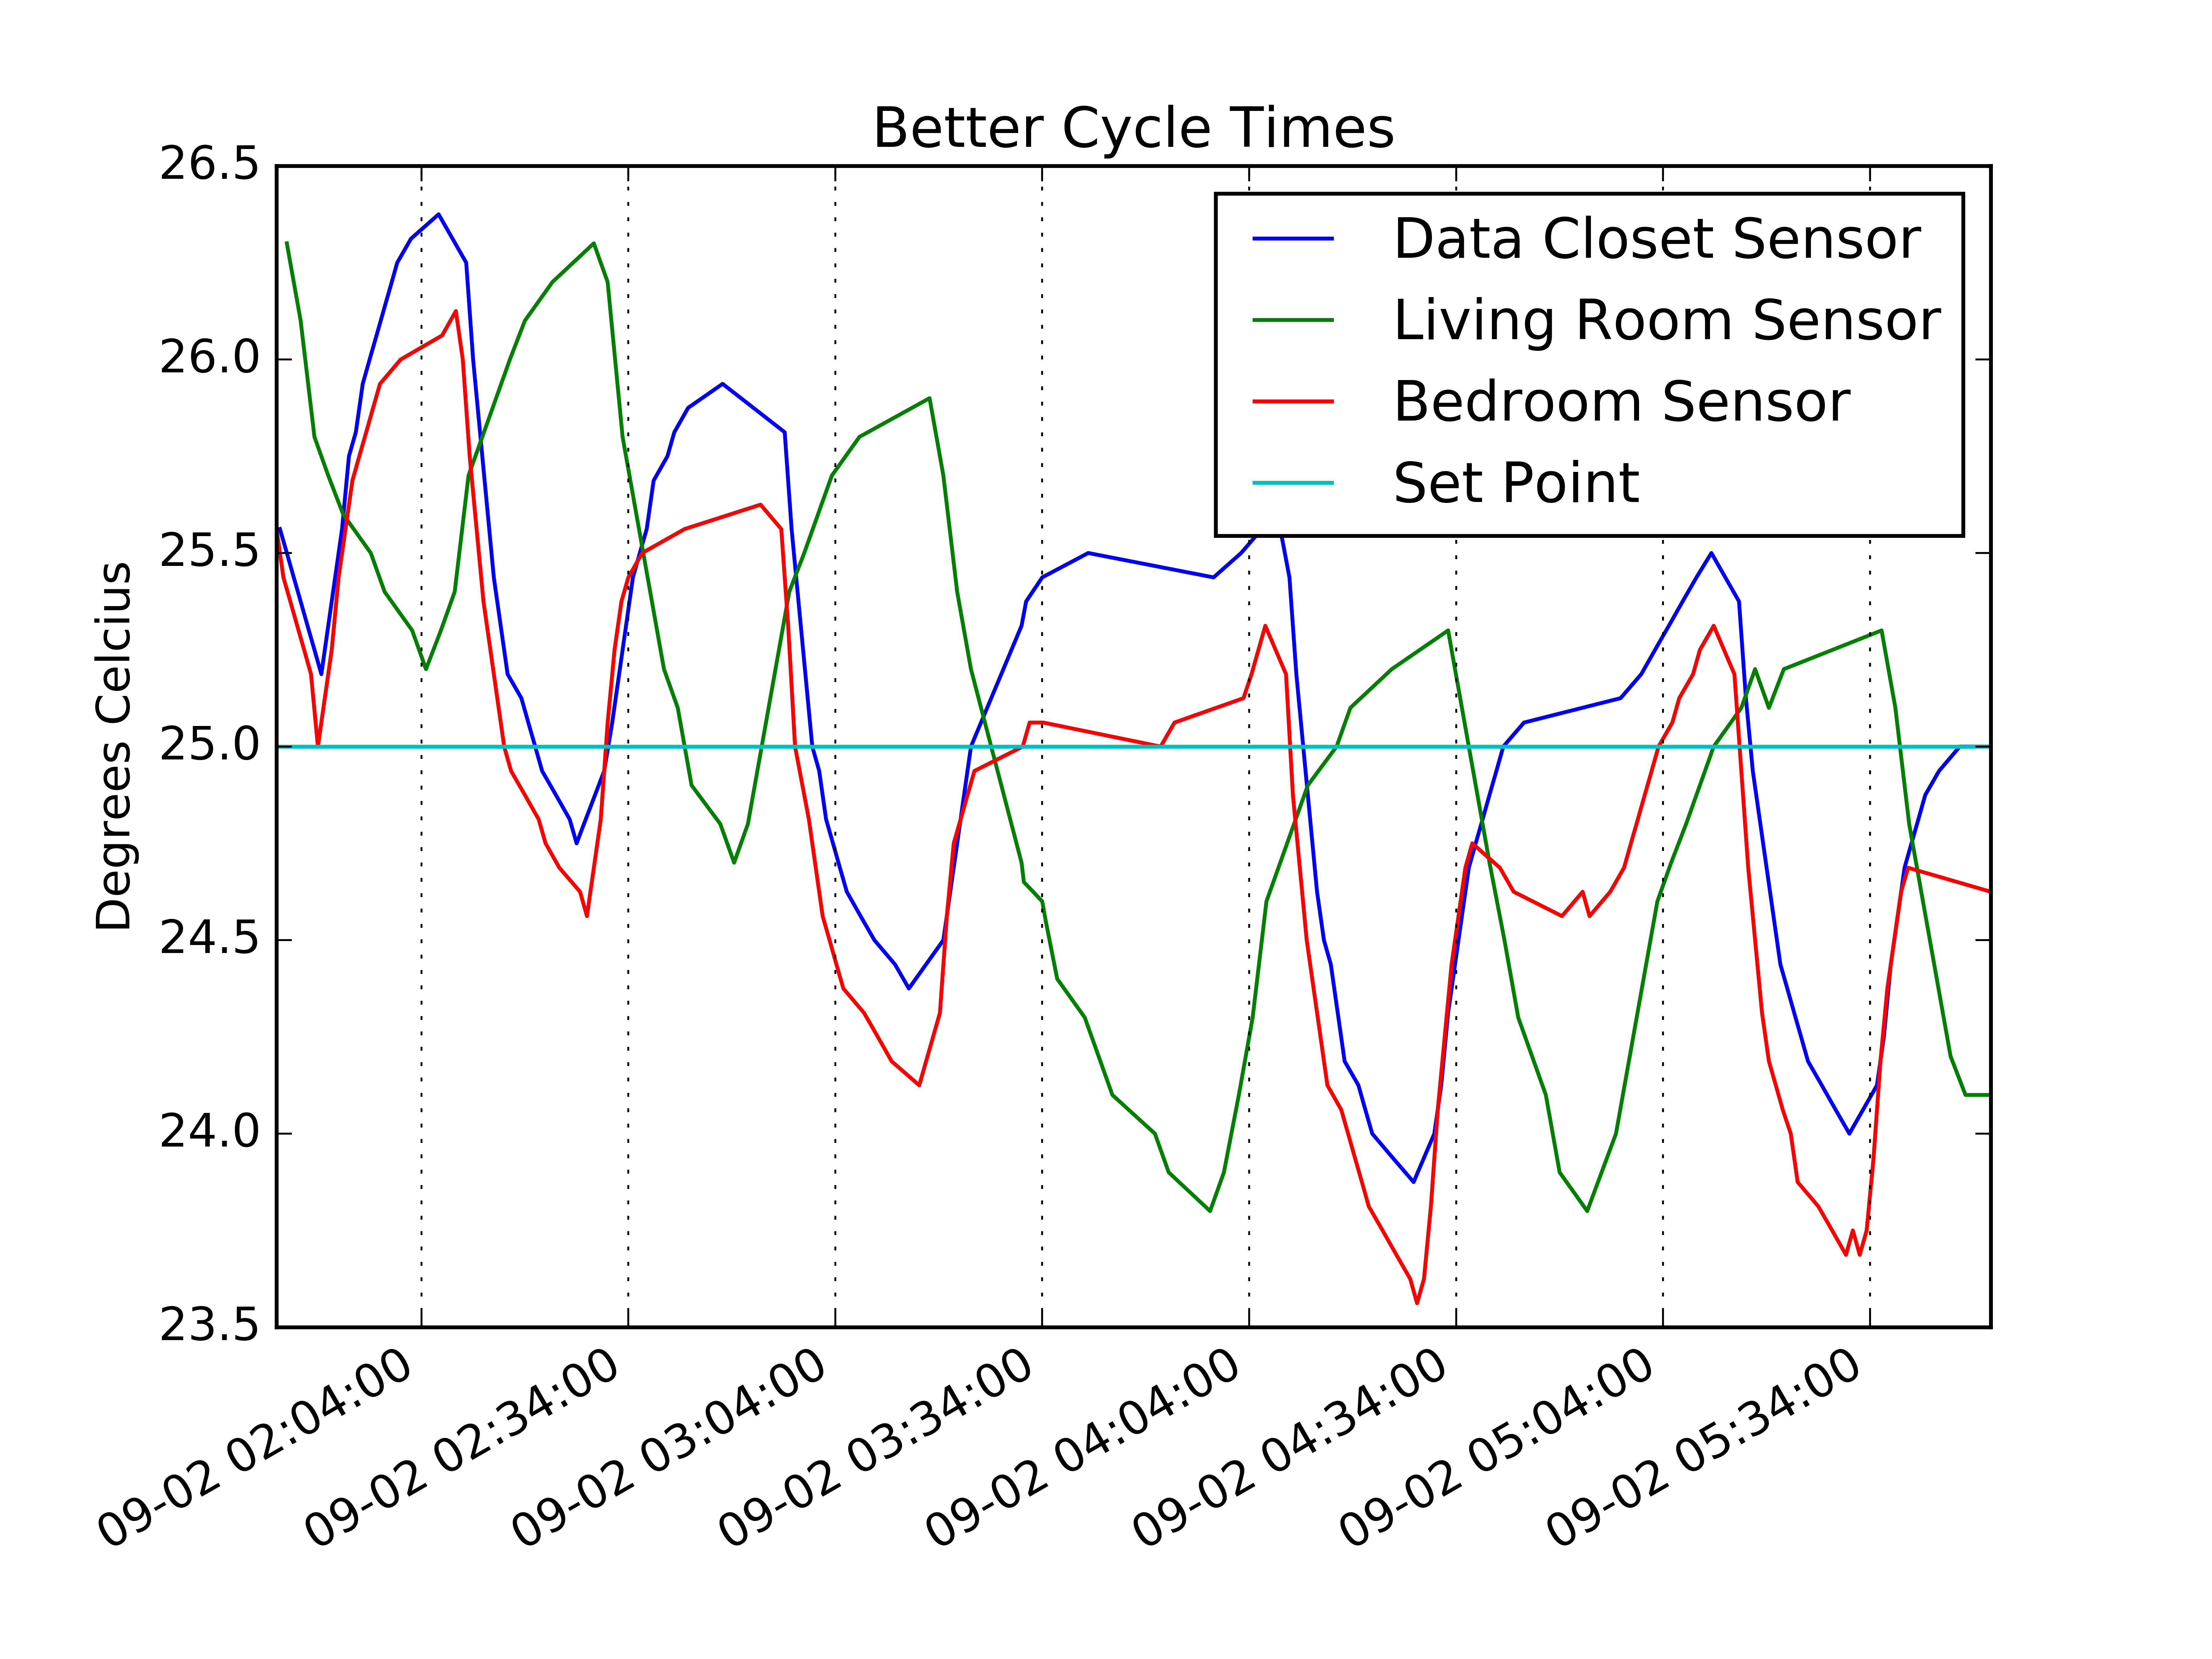
\includegraphics[height=.75\textheight]{long_cycle.png}
    \end{center}
    \begin{itemize}
        \item Bedroom on for 20 min. and off for 21 min.
        \item Living Room on for 17 min. off for 29 min.
    \end{itemize}
\end{frame}

\section{Automation}
\begin{frame}[fragile=singleslide]
    \frametitle{Starting to Automate}
    \begin{minted}[
      gobble=4,
      frame=single,
      linenos
    ]{yaml}
      alias: Set Living Room AC to 30 C when asleep
      trigger:
        platform: time
        after: '12:30:00'
      condition:
        - condition: time
          before: '09:30:00'
      action:
        service: thermostat.set_temperature
        entity_id: thermostat.living_room
        data:
          temperature: 30
    \end{minted}
\end{frame}

\subsection{Location based rules}
\begin{frame}
    \frametitle{Location Tracking}
    \begin{itemize}
        \item Start writing rules based on my location
        \item Set temperature higher when I'm not home
        \item Pre-cool apartment when I'm heading home
    \end{itemize}
\end{frame}

\begin{frame}
    \frametitle{Owntracks}
    \begin{columns}[T]
        \begin{column}{.48\textwidth}
            \begin{itemize}
                \item Open Source iOS and Android app for reporting location over MQTT
                \item Enables you to use either a private MQTT broker or public service
                \item Home Assistant component available
            \end{itemize}
        \end{column}
        \begin{column}{.48\textwidth}
            \centering
            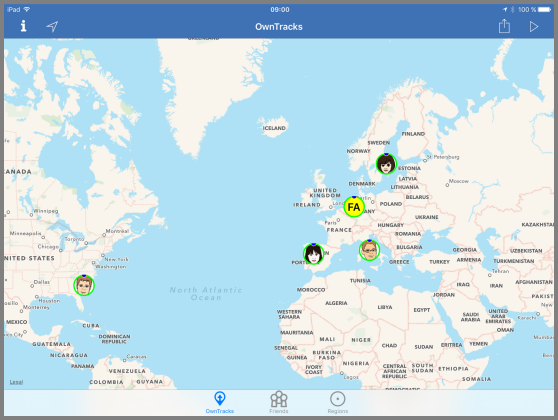
\includegraphics[width=.8\textwidth]{ipad-public-map.png}
        \end{column}
    \end{columns}
\end{frame}

\begin{frame}[fragile=singleslide]
    \frametitle{Location Based Automation Rules}
    \begin{minted}[
      gobble=4,
      frame=single,
      linenos
    ]{yaml}
        alias: Set Living Room AC to 26 C when leaving starbucks route 9
        trigger:
          platform: state
          entity_id: device_tracker.myphone
          from: 'Starbucks Route 9'
        action:
          - delay:
              minutes: 5
          - service: climate.set_temperature
            entity_id: climate.living_room
            data:
              temperature: 26
    \end{minted}
\end{frame}

\subsection{Environment Based Conditions}
\begin{frame}[fragile=singleslide]
    \frametitle{Turn the Air Conditioning off Based on the Outside Temperature}
    \begin{minted}[
      gobble=4,
      frame=single,
      linenos
    ]{yaml}
      alias: Turn off AC when it's cold outside
      trigger:
        platform: numeric_state
        entity_id: sensor.pws_temp_c
        below: 22.0
      action:
        service: thermostat.set_operation_mode
        entity_id: thermostat.living_room
        data:
          operation_mode: off
    \end{minted}
\end{frame}

\begin{frame}[fragile=singleslide]
    \frametitle{Increase TV volume when the AC turns on}
    \begin{minted}[
      gobble=4,
      frame=single,
      linenos
    ]{yaml}
      alias: Raise volume when AC turns on
      trigger:
        platform: state
        entity_id: switch.aeotec_zw096_smart_switch_6_switch_2_0
        to: 'on'
      conditions:
        - condition: state
          entity_id: media_player.living_room_av_reciever
          state: 'on'
        - condition: template
          value_template: '{{ states.media_player.reciever.volume_level < 0.7 }}'
      action:
        service: media_player.volume_up
        entity_id: media_player.living_room_av_reciever
    \end{minted}
\end{frame}

\begin{frame}[fragile=singleslide]
    \frametitle{Turn AC on when Closet Cloud starts}
    \begin{minted}[
      gobble=4,
      frame=single,
      linenos
    ]{yaml}
      alias: Turn AC on when altocumulus starts
      trigger:
        platform: state
        entity_id: switch.altocumulus01
        from: 'off'
        to: 'on'
        for:
           minutes: 2
      action:
        service: climate.set_operation_mode
        entity_id: climate.bedroom
        data:
          operation_mode: on
    \end{minted}
\end{frame}

\begin{frame}
    \frametitle{Future Work}
    \begin{itemize}
        \item More Sensors
        \item More automation
        \item Additional Power monitoring
        \item Adjust/tune switching parameters
    \end{itemize}
\end{frame}

\section{Questions?}
\begin{frame}
\frametitle{Where to get more information}
    \begin{itemize}
        \item Blog Post \href{http://blog.kortar.org/?p=319}{http://blog.kortar.org/?p=319}
        \item \href{https://home-assistant.io/}{https://home-assistant.io/}
        \item \href{https://github.com/mtreinish/dallasMQTT}{https://github.com/mtreinish/dallasMQTT}
        \item \href{http://zwavepublic.com/}{http://zwavepublic.com/}
        \item \href{http://owntracks.org/}{http://owntracks.org/}
        \item \href{https://github.com/openzwave/}{https://github.com/openzwave/}
        \item W.J. Mulroy, ``The Effect of Short Cycling and Fan Delay on the Efficiency of a Modified Residential Heat Pump``, \textit{ASHRAE Transactions}, Vol. 92, No. Part 1, pp. 813-816, January 1986
        \item Slides: \href{https://github.com/mtreinish/building-a-better-thermostat/tree/lca2018}{https://github.com/mtreinish/building-a-better-thermostat/tree/lca2018}
    \end{itemize}
\end{frame}

\end{document}
